\documentclass[11pt,a4paper]{article}

\usepackage[margin=1in]{geometry}
\usepackage[T1]{fontenc}
\usepackage[utf8]{inputenc}
\usepackage{lmodern}
\usepackage{microtype}
\usepackage{booktabs}
\usepackage{amsmath}
\usepackage{enumitem}
\usepackage[hidelinks]{hyperref}

\title{Household Fuel Price Risk and the Uneven Protective Value of Domestic Net Zero: Evidence from Westminster, London}
\author{}
\date{\today}

\begin{document}
\maketitle

\begin{abstract}
Fuel poverty identifies current affordability hardship, but it does not by itself measure future household exposure to fossil-fuel price shocks. This paper develops the concept of household fuel price risk and applies it to Westminster, London, using property-level or property-archetype modelling. The empirical strategy estimates required energy demand, baseline energy burden, price-shock sensitivity, and the distributional effect of domestic low-carbon interventions. The central argument is that domestic net zero is not automatically a household risk-protection strategy. Retrofit, clean heat, solar PV, battery storage, smart tariffs, and flexibility reduce unequal exposure only when housing fabric, heating systems, tariff design, market reform, tenure, and local governance align.
\end{abstract}

\noindent\textbf{Keywords:} fuel poverty; energy burden; price risk; domestic retrofit; net zero; Westminster; energy justice

\section{Introduction}

Fuel poverty research has made household energy hardship visible, but the recent politics of domestic energy requires a further question. A household may not be classified as fuel poor at one point in time and yet remain highly exposed to the next fossil-fuel price shock; equally, a household may receive a low-carbon technology without receiving meaningful protection from volatile retail energy costs. This paper therefore reframes household energy inequality from a static problem of current fuel poverty into a dynamic problem of uneven exposure to future fossil-fuel price volatility.
% Citation TODO: fuel poverty metrics, energy vulnerability, energy price resilience.

This reframing is significant for three reasons. First, energy-price shocks are not merely temporary deviations from a normal affordability problem. They reveal which households have high required energy needs, thin residual incomes, limited ability to absorb bill increases, and little control over the building or tariff conditions that shape their exposure. Second, actual expenditure can understate hardship when households respond to high prices by underheating, self-rationing, or delaying payment. A risk framework must therefore start from required energy services and then ask how costs change under plausible price and policy scenarios. Third, domestic net zero is increasingly presented as a route to lower bills and improved resilience, but the household-protection effect is not automatic. It depends on whether technical change reduces required demand, changes the household's fuel-price exposure, and is accessible under the household's tenure, dwelling form, tariff options, and local governance constraints.
% Citation TODO: underheating/required expenditure; retrofit and net-zero policy claims; tariff and price-shock literature.

Existing studies provide important building blocks but do not fully answer this paper's question. Fuel poverty indicators identify current need and support policy targeting, while energy vulnerability research shows that hardship is produced through income, housing quality, health, tenure relations, social support, and institutional access. Recent work on energy price resilience, energy poverty premiums, underheating, and crisis-period demand reduction moves closer to household price-risk analysis. Retrofit and low-carbon technology studies also show that fabric improvements, heat pumps, PV, batteries, and flexibility can alter energy demand and bills. Yet these literatures often remain separated: fuel poverty metrics are usually current-condition indicators; retrofit studies often focus on average energy or bill effects; low-carbon adoption research examines who installs technologies more than who receives price-risk protection; and price-shock studies rarely connect future volatility to local housing governance and intervention feasibility at property or small-area scale.
% Citation TODO: fuel poverty indicators; energy vulnerability; household energy price resilience; low-carbon adoption inequality; retrofit evaluation.

The gap is especially important in the United Kingdom because decarbonisation and de-risking can diverge. Electrification can reduce direct household gas use and emissions, but it may not reduce household fuel price risk if electricity prices remain high relative to gas or continue to transmit gas-market shocks through wholesale and retail bill structures. Similarly, PV, batteries, and smart tariffs may hedge electricity-price exposure for some households while excluding others because of roof access, leasehold governance, smart-meter access, digital capability, load flexibility, or capital cost. The policy question is therefore not whether a measure is low carbon in engineering terms, but whether it reduces upper-tail household burden risk for the households most exposed to price volatility.
% Citation TODO: UK electricity-gas price ratio, gas pass-through, smart tariff equity, PV/battery access.

Westminster is an analytically revealing case rather than a merely convenient location. High average wealth can obscure fuel-price vulnerability among households facing high housing costs, inefficient or hard-to-retrofit dwellings, private rental constraints, leasehold governance, heritage restrictions, and limited access to low-carbon assets. Dense flats, social housing blocks, private rented weak-fabric dwellings, electric-heated inefficient flats, large inefficient gas-heated homes, and conservation-area properties create different routes into exposure and different routes out of it. These conditions make Westminster a strong test of whether domestic net zero can operate as household price-risk protection, and for whom.
% Citation TODO: Westminster/London housing, retrofit, PRS, heritage, fuel poverty evidence.

The paper's starting point is therefore not that domestic net zero measures are inherently protective. A dwelling can become lower carbon without becoming less exposed to household price risk if the intervention leaves required heat demand high, shifts the household onto a more expensive fuel, excludes the occupant from favourable tariffs, or depends on building-level decisions outside the household's control. Conversely, the same intervention may be protective where fabric improvement, heating-system efficiency, tariff design, finance, and governance align. The key distributional question is who receives this protection and who remains exposed.

The central research question is: to what extent, and under what housing, market, and governance conditions, do domestic net zero interventions reduce unequal household exposure to fossil-fuel price volatility in Westminster?

The paper addresses three linked questions:
\begin{enumerate}[label=\arabic*.]
    \item Which household-dwelling types face the largest required energy burden increase under fuel price shocks?
    \item How do income, housing fabric, heating system, tenure, and vulnerability jointly produce fuel price risk?
    \item How much risk reduction do retrofit, clean heat, PV, battery storage, smart tariffs, and integrated packages deliver, and for whom?
\end{enumerate}

The contribution is fourfold. Conceptually, the paper distinguishes fuel poverty as current hardship, energy burden as a cost-to-income relation, and household fuel price risk as future-facing exposure, sensitivity, and limited adaptive capacity under price-shock scenarios. Methodologically, it develops a transparent income--cost and scenario framework that links required energy demand, local residual-income distributions, fuel-price shocks, intervention feasibility, and upper-tail burden risk. Empirically, it applies this framework to Westminster's heterogeneous housing stock, where high-cost urban housing, tenure governance, flats, heritage constraints, and social housing delivery pathways are central mechanisms rather than contextual details. For policy, it evaluates domestic net zero interventions as conditional de-risking tools, not as automatic bill-reduction or emissions-reduction proxies.

The modelling strategy follows directly from this argument. The baseline layer estimates required energy burden and the probability of crossing a burden threshold, because these measures identify where current cost and income conditions make exposure plausible even without observing each occupant's income. The price-shock layer then varies fuel prices, standing charges, tariff structures, and mitigation to estimate how exposure changes under future conditions. The intervention layer finally asks whether fabric retrofit, clean heat, PV, storage, smart tariffs, or integrated packages reduce upper-tail burden risk once access constraints are included. The equations are therefore not a detached technical apparatus; they are the operational form of the paper's central claim that current hardship, future exposure, and conditional protection must be measured separately before their distribution can be compared.

\section{Conceptual Framework}

The paper separates three concepts that are often conflated. Fuel poverty identifies present affordability hardship under current prices and required energy needs. Energy burden measures required or actual energy cost relative to residual household income. Household fuel price risk captures future exposure, sensitivity, and limited adaptive capacity under price-shock scenarios.

\begin{equation}
\text{Household fuel price risk} = \text{exposure} + \text{sensitivity} - \text{adaptive capacity}.
\end{equation}

The implemented baseline burden indicators should therefore be read as current-price affordability measures, not as the final fuel-price-risk outcome. They provide the income--cost foundation for later shock scenarios, but they do not themselves represent future exposure unless fuel-price, tariff, and intervention counterfactuals are introduced.

In the empirical work, this distinction is operationalised through two related but non-equivalent burden measures. The first is a deterministic baseline required-energy-burden ratio: SAP-derived required energy cost divided by MSOA after-housing-cost disposable income. The second is a probabilistic threshold measure: the probability that a household drawn from the property's LSOA income distribution would face a required energy burden above 10 percent. The former is intuitive as a cost-to-income ratio; the latter is better suited to identifying local income-tail exposure. Neither measure is an official fuel-poverty classification, and neither should be read as future household fuel price risk before price shocks are modelled.

This matters for interpretation. A top-decile modelled burden-risk group identifies the high end of Westminster's current required-cost and income-distribution assumptions. It does not mean that every property in that group is occupied by a verified fuel-poor household, nor that all other properties are protected. Instead, it marks where required energy demand, local income sensitivity, and dwelling characteristics make high burden more probable under current prices. The future-facing risk analysis must then ask how this baseline exposure changes when gas prices, electricity prices, standing charges, tariff access, and policy mitigations are varied.

This distinction matters because decarbonisation is not the same as de-risking. Electrification can reduce emissions before it reduces household price risk where electricity prices remain linked to gas through wholesale market design. The protective value of heat pumps, PV, storage, smart tariffs, and flexibility therefore depends on the electricity-gas price ratio, tariff access, capital access, dwelling form, tenure, and governance.

\section{Case and Data}

The empirical case is Westminster, London. The preferred unit of analysis is the property or household-dwelling pair. Where household microdata are unavailable, the study uses EPC property records combined with LSOA/MSOA income and deprivation proxies to assign synthetic households or archetypes.

The current enriched property master contains 124,980 properties across 126 LSOAs and 26 MSOAs. It combines EPC attributes, spatial identifiers, MSOA after-housing-cost income, LSOA income deprivation, official LSOA fuel poverty rates, and LSOA income-distribution outputs from the latest verified pipeline.

The analysis uses required energy demand rather than only observed expenditure, because actual consumption may understate unmet need through underheating or self-rationing.

\section{Methods}

The empirical strategy is a property-level income--cost and scenario model. It links EPC-derived dwelling characteristics, synthetic LSOA income distributions, required energy costs, price-shock scenarios, domestic net zero intervention packages, and spatial-distributional outputs. The unit of analysis is property $p$ in LSOA $l$ and MSOA $m$. Where observed household incomes are unavailable, the model estimates the probability that a household drawn from the local residual-income distribution would face a given required-energy burden. This design is deliberately probabilistic: it does not claim to observe the income of the current occupant of each property.

The equations are chosen to match the conceptual problem rather than to maximise statistical complexity. The paper needs a model that can do four things transparently: estimate required energy affordability under current conditions; expose the same property-income combinations to future fuel-price shocks; distinguish average burden from upper-tail burden risk; and compare intervention packages only after technical, tenure, tariff, and governance constraints are represented. A property-level scenario model is appropriate because the key mechanisms operate at different scales: dwelling fabric and heating systems are property-level, income distributions are small-area approximations, tariffs and fuel prices are market-level, and feasibility constraints are mediated by tenure, leasehold, heritage, and local delivery. The model is therefore not a prediction of exact bills for named households. It is a structured counterfactual framework for asking which property--income--governance combinations are most exposed and which interventions reduce that exposure.

This approach is also deliberately modular. The income--cost engine establishes the baseline denominator and required-cost numerator. The price-shock engine changes unit prices, standing charges, and mitigation while holding the logic of required demand explicit. The intervention engine then changes demand, fuel structure, tariff access, and feasibility. Because each layer modifies a different part of the same burden equation, the resulting de-risking estimates remain interpretable: a lower risk score can be traced to lower required demand, lower unit-price exposure, improved tariff access, policy support, or greater feasibility. This is why the equations are sufficient for the paper's purpose even though they do not observe all household behaviours directly.

\subsection{Income--Cost Engine}

The income--cost engine answers the first empirical problem: how can current required-burden exposure be estimated when the dataset contains properties rather than verified household incomes? A single average income would suppress Westminster's local lower tail, while assigning one synthetic income to each property would imply false precision. The constrained lognormal specification provides a middle route. It keeps MSOA after-housing-cost income as an anchor, allows LSOA-level lower-tail differentiation through deprivation information, and returns probabilities rather than definitive household labels.

The implemented income layer estimates one constrained lognormal after-housing-cost income distribution for each LSOA:
\begin{equation}
Y_l \sim \operatorname{Lognormal}(\mu_l,\sigma_l^2),
\end{equation}
where $Y_l$ denotes annual residual household income. The distribution is parameterised by its mean $\bar{Y}_l$:
\begin{equation}
\mu_l=\ln(\bar{Y}_l)-\frac{1}{2}\sigma_l^2 .
\end{equation}
For each MSOA, the LSOA parameters are jointly estimated so that the property-weighted mean remains anchored to the MSOA after-housing-cost income, while the lower tail is differentiated by the LSOA income-deprivation signal. The LSOA income-deprivation term is treated as a robust soft constraint on the lower tail, not as an equality target. For a given regularisation parameter $\lambda$, the current objective is:
\begin{equation}
\begin{split}
\mathcal{L}_m(\lambda)=&
\left[
\ln \left(\frac{\sum_{l \in m} N_l \bar{Y}_l}{\sum_{l \in m} N_l}\right)
-\ln(\bar{Y}_m)
\right]^2 \\
&+\lambda \sum_{l \in m} w_l
\rho_{\eta}\left(F_l(z)-d_l\right),
\end{split}
\end{equation}
where $N_l$ is the number of EPC property records in LSOA $l$, $w_l=N_l/\sum_{l \in m}N_l$, $\bar{Y}_m$ is MSOA residual income, $z=19{,}009$ is the income threshold used in the current module, $F_l(\cdot)$ is the LSOA lognormal cumulative distribution function, and $d_l$ is the LSOA income-deprivation score. The robust loss is the pseudo-Huber L1 form:
\begin{equation}
\rho_{\eta}(d)=\sqrt{d^2+\eta^2}-\eta,
\qquad \eta=10^{-3}.
\end{equation}
The fixed $\eta$ is a numerical differentiability regulariser for optimisation rather than a substantive research parameter. The current implementation constrains $\sigma_l \in [0.10,1.40]$ and searches a log-spaced grid of 100 $\lambda$ values from $10^{-4}$ to $10^{-1}$. Official LSOA fuel-poverty rates are used only as an external diagnostic to select $\lambda$ by minimising property-weighted RMSE, with weighted MAE and then the larger $\lambda$ as tie-breakers; they are not entered directly as the optimisation target.

The May 2026 sensitivity run also varies the MSOA after-housing-cost income anchor across central, upper-confidence-limit, and lower-confidence-limit scenarios. These scenarios bracket income-anchor uncertainty for the baseline burden model. They are not income forecasts, and they do not replace the canonical property-level master until a deliberate rerun is approved.

Required energy cost is derived from SAP and floor area rather than from observed consumption, because actual expenditure may be suppressed by underheating or self-rationing. For property $p$, the SAP energy cost factor is:
\begin{equation}
\operatorname{ECF}_p=
\begin{cases}
(100-\operatorname{SAP}_p)/16.21, & \operatorname{SAP}_p \geq 43.265,\\
10^{(108.8-\operatorname{SAP}_p)/120.5}, & \operatorname{SAP}_p < 43.265.
\end{cases}
\end{equation}
The baseline required annual energy cost is then:
\begin{equation}
C_{p,0}=\operatorname{ECF}_p \frac{A_p+45}{0.2},
\end{equation}
where $A_p$ is total floor area. Baseline required energy burden for a household with income $Y_l$ is:
\begin{equation}
B_{p,0}(Y_l)=\frac{C_{p,0}}{Y_l}.
\end{equation}
The current module therefore estimates burden-threshold probabilities:
\begin{equation}
P_{p,0}(\tau)=\Pr \left(B_{p,0}(Y_l)>\tau \right)
=F_l\left(\frac{C_{p,0}}{\tau}\right).
\end{equation}
The implemented baseline output uses $\tau=0.10$. For modelled LSOA fuel-poverty comparison, properties with SAP grades A, B, or C are assigned a property poverty score of zero; other properties use $P_{p,0}(0.10)$. This score is a baseline affordability input, not a complete measure of household fuel price risk.

The threshold probability is useful because it reports exposure to a policy-relevant affordability boundary without claiming that the boundary is the whole concept of fuel poverty. It also avoids reducing Westminster's mixed-income geography to area averages. A property can have moderate deterministic burden under the MSOA mean but still have a substantial probability of high burden for households in the local lower tail. Conversely, a property with high required cost may be less probabilistically exposed if local residual incomes are high. This distinction is central to the paper's question because price shocks will interact with both required demand and income sensitivity.

The residual gap between the modelled poverty proxy and official LSOA fuel-poverty rates is interpreted as a limitation of construct alignment rather than as a simple tuning failure. Income deprivation, required-energy burden, and official fuel poverty are related but non-equivalent measures. Under the current parameterisation, the MSOA mean term anchors $\bar{Y}_l$, while the LSOA lower-tail term strongly identifies $\sigma_l$; changing the lower-tail loss from squared error to pseudo-Huber L1 therefore did not materially change the fitted distributions. This is useful diagnostically because it cautions against using official fuel poverty as if it were the same object as income-tail exposure or future fuel price risk.

For robustness, the pipeline also reports a deterministic baseline burden ratio:
\begin{equation}
\widetilde{B}_{p,0}=\frac{C_{p,0}}{\bar{Y}_m},
\end{equation}
where $\bar{Y}_m$ is the MSOA after-housing-cost income point estimate. This measure is easier to interpret as a cost-to-income ratio, but it does not model within-LSOA income dispersion and is not calibrated to the local fuel-poverty comparison.

\subsection{EPC Enrichment and High-Risk Pathways}

The latest explanatory layer enriches the Westminster property master with EPC certificate records using UPRN-based linkage. UPRNs are standardised before both merging and QA checks, so that numeric and string representations of the same property identifier do not generate false unmatched cases. Where multiple EPC certificates are available for a property, the selected record is the latest \texttt{LODGEMENT\_DATETIME}; where this is unavailable, the latest \texttt{INSPECTION\_DATE} is used, and remaining ties fall back to the first available row. EPC fields are added with an \texttt{EPC\_} prefix, the original property master is not overwritten, and the row count and row order of the master are preserved.

The enrichment is followed by an explicit audit stage covering unmatched master records, duplicate UPRNs, added-field missingness, EPC rating distributions, lodgement-year distributions, and original versus corrected tenure groups. The EPC-derived tenure variable is treated as a proxy for tenure-related adaptive capacity rather than as observed legal tenure. The analysis version, \texttt{EPC\_TENURE\_GROUP\_FIXED}, classifies social rented records before private rented records to avoid misclassifying social rental descriptions as private rental cases.

The enriched stock is then transformed into a descriptive high-risk layer. Derived variables capture EPC performance, SAP-derived required energy cost, fabric weakness, electric heating exposure, gas connection, corrected tenure proxy, baseline required energy burden, and membership in modelled high-burden groups. The main current-condition groups are the top decile and top quintile of $P_{p,0}(0.10)$, denoted HR10 and HR20. Robustness groups use the top decile and top quintile of deterministic baseline required energy burden, denoted BR10 and BR20; an additional deterministic threshold group identifies properties with $\widetilde{B}_{p,0}>0.10$. These groups describe current modelled burden probability and required-burden intensity; they are not official fuel-poverty classifications and do not by themselves constitute the future-facing household fuel price risk measure.

The distinction between HR and BR groups is analytically useful rather than merely technical. HR groups identify properties whose required costs interact with the local LSOA income distribution to produce a high probability of crossing a 10 percent burden threshold. BR groups identify properties with high deterministic required burden relative to the MSOA point estimate of after-housing-cost income. Their overlap is therefore expected to be partial: the two approaches should identify a related high-burden tail, while also showing whether income-distribution assumptions change who is treated as exposed.

Finally, high-risk properties are assigned to mutually exclusive descriptive pathways using priority rules. The current typology distinguishes inefficient large owner-occupied gas houses, social rented estate or block risk, private rented weak-fabric gas flats, electric-heated inefficient flats or maisonettes, high-demand inefficient maisonettes, and a residual high-risk group. The pathway typology is not a causal model. Its purpose is to provide an interpretable bridge between property-level burden modelling and the later price-shock and intervention simulations, so that de-risking outcomes can be reported by mechanism and governance pathway rather than only for the aggregate stock.

The corresponding descriptive figures report pathway risk and contribution, EPC--floor-area sensitivity, tenure structure, electric exposure, spatial concentration, and HR--BR overlap (Figures~\ref{fig:hr-br-overlap}--\ref{fig:spatial-high-risk}). They are current-condition burden-exposure diagnostics rather than price-shock results.

\subsection{Price-Shock Risk Metrics}

The price-shock layer converts the baseline income--cost engine into forward-looking risk metrics. Let $s \in S$ denote a fuel-price scenario, including gas-price, electricity-price, combined-fuel, standing-charge, and policy-mitigation cases. Required cost under scenario $s$ is written as:
\begin{equation}
C_{p,s}=\pi^g_s Q^g_p+\pi^e_s Q^e_p+SC^g_s I^g_p+SC^e_s I^e_p-M_{p,s},
\end{equation}
where $Q^g_p$ and $Q^e_p$ are required gas and electricity quantities or archetype-imputed equivalents, $\pi^g_s$ and $\pi^e_s$ are scenario fuel prices, $SC^g_s$ and $SC^e_s$ are standing charges, $I^g_p$ and $I^e_p$ indicate fuel connections, and $M_{p,s}$ captures bill support or other mitigation. The scenario burden is:
\begin{equation}
B_{p,s}(Y_l)=\frac{C_{p,s}}{Y_l},
\end{equation}
and the burden uplift is:
\begin{equation}
\Delta B_{p,s}(Y_l)=B_{p,s}(Y_l)-B_{p,0}(Y_l).
\end{equation}

This cost equation is intentionally simple and explicit. It separates the components through which price risk reaches households: gas unit prices, electricity unit prices, fixed standing charges, fuel connections, and policy mitigation. That separation is necessary because different interventions act on different terms. Fabric retrofit reduces required quantities; heat pumps change the gas-electricity mix; PV and batteries reduce grid electricity imports under some profiles; tariff reform changes prices or standing charges; and public support enters as mitigation. A more compact total-bill equation would obscure these mechanisms and make it harder to explain why an intervention protects one group but not another.

The main risk indicators are defined as distributional rather than average outcomes. The scenario-specific threshold-crossing probability is:
\begin{equation}
P_{p,s}(\tau)=F_l\left(\frac{C_{p,s}}{\tau}\right).
\end{equation}
For scenario weights $\omega_s$, the expected threshold-crossing risk is:
\begin{equation}
R_{p}(\tau)=\sum_{s \in S}\omega_s P_{p,s}(\tau).
\end{equation}
An affordability gap-at-risk can be expressed as the expected shortfall above an acceptable burden threshold:
\begin{equation}
G_{p,s}(\tau)=\operatorname{E}_{Y_l}\left[\max\{C_{p,s}-\tau Y_l,0\}\right].
\end{equation}
Household Fuel Price-at-Risk is defined as a high quantile of the scenario burden distribution:
\begin{equation}
\operatorname{HFPaR}_{p,\alpha}
=\inf \left\{b:\sum_{s \in S}\omega_s \mathbf{1}\left(B_{p,s}\leq b\right)\geq \alpha \right\},
\end{equation}
where $\alpha$ may be set to a policy-relevant upper-tail level such as 0.90 or 0.95. These metrics keep fuel poverty, energy burden, and fuel price risk analytically separate: the first concerns current hardship, the second is a cost-to-income ratio, and the third measures future exposure and sensitivity under price shocks.

The three risk metrics have different policy uses. Threshold-crossing probabilities show how many property-income combinations are likely to move beyond an affordability boundary. Gap-at-risk reports the monetary depth of exposure above that boundary, which matters for bill support or social tariff design. Household Fuel Price-at-Risk focuses on the upper tail of the scenario burden distribution, which is the relevant object when the policy concern is protection against shocks rather than average annual affordability. Reporting all three avoids a false choice between headcount, severity, and tail-risk interpretations.

\subsection{Intervention Counterfactuals}

Domestic net zero interventions are represented as counterfactual changes to required demand, fuel structure, tariff exposure, and mitigation access. Let $k$ denote an intervention package, such as fabric retrofit, clean heat, PV, battery storage, smart tariffs, or an integrated package. The post-intervention scenario cost is:
\begin{equation}
C_{p,s,k}=
a_{p,k}\widetilde{C}_{p,s,k}+(1-a_{p,k})C_{p,s},
\end{equation}
where $a_{p,k}\in[0,1]$ represents technical, tenure, leasehold, heritage, roof, finance, or tariff feasibility. This term is central to the paper's interpretation: an intervention produces household risk protection only where access and market conditions allow the technical change to translate into lower exposure.

The feasibility parameter is not a decorative adjustment. It is the formal expression of the paper's claim that domestic net zero is conditional household protection. Without $a_{p,k}$, the model would implicitly assume that every property can receive every intervention and that all occupants can capture the resulting benefit. That assumption would be especially misleading in Westminster, where flats, leasehold blocks, private renting, social housing delivery, heritage constraints, roof rights, smart-meter access, and tariff eligibility all shape whether an engineering option becomes a household de-risking option.

The intervention-specific threshold risk and Fuel Price-at-Risk are:
\begin{equation}
P_{p,s,k}(\tau)=F_l\left(\frac{C_{p,s,k}}{\tau}\right),
\qquad
\operatorname{HFPaR}_{p,\alpha,k}
=Q_{\alpha}\left(\{B_{p,s,k}\}_{s \in S}\right).
\end{equation}
The de-risking dividend is the reduction in upper-tail burden risk:
\begin{equation}
D_{p,\alpha,k}=
\operatorname{HFPaR}_{p,\alpha,0}
-
\operatorname{HFPaR}_{p,\alpha,k}.
\end{equation}
Results will be stratified by income distribution, EPC rating, dwelling form, heating system, tenure, leasehold and heritage constraints, and LSOA/MSOA location. The empirical question is therefore not whether a low-carbon measure reduces emissions in engineering terms, but who receives measurable price-risk protection once required demand, tariffs, fuel-market pass-through, and local governance constraints are jointly considered.

The de-risking dividend is the bridge between the conceptual and empirical contributions. It does not ask whether an intervention is technically impressive on average. It asks whether the intervention reduces the upper-tail burden that households would face across price-shock scenarios. A positive dividend means that the package has converted at least part of the technical or policy change into lower household price-risk exposure. A small or uneven dividend indicates either that the intervention does not affect the relevant risk channel, or that feasibility, tariff access, price pass-through, or income sensitivity prevents households from capturing the protection.

\section{Expected Outputs}

The empirical outputs are designed to move from an implemented income--cost baseline to forward-looking price-risk and intervention comparisons. The latest canonical property-level modelling round already provides the first layer of this sequence: a baseline required-energy-burden engine for Westminster, built from constrained LSOA income distributions and SAP-derived required energy costs. The run labelled \texttt{20260520\_213323} covers 124,980 EPC property records across 126 LSOAs and 26 MSOAs. It preserves MSOA after-housing-cost income consistency while allowing LSOA differentiation mainly through income dispersion and lower-tail probability, rather than by claiming directly observed household incomes. A subsequent read-only sensitivity run labelled \texttt{20260526\_144256} tests alternative MSOA income anchors and the pseudo-Huber L1 lower-tail constraint; it is used here as a robustness diagnostic rather than as a replacement for the canonical property-level master.

\subsection{Implemented Baseline Outputs}

The current outputs support three baseline products. First, the model estimates LSOA lognormal income parameters, including $\mu_l$, $\sigma_l$, lower-tail probabilities below \pounds 19{,}009, and the selected MSOA-level regularisation parameter $\lambda$. In the canonical verified run, the ratio of LSOA mean income to MSOA income is tightly anchored, ranging from 0.999650 to 1.000309, while $\sigma_l$ ranges from 0.4192 to 1.4000. Only 3 of 126 LSOAs sit at the new upper bound, compared with 31 of 126 under the previous bound of 0.9. This indicates that within-MSOA differentiation is being carried primarily by dispersion and tail probability.

Second, the model produces property-level SAP-derived required energy cost and the probability that required energy burden exceeds a 10 percent threshold. This output should be interpreted as baseline required-energy affordability exposure, not as a complete household fuel price risk measure. It provides the denominator and cost foundation for later shock scenarios, while avoiding dependence on actual expenditure that may be suppressed by underheating or self-rationing.

The 2026-05-28 baseline extract turns this layer into a fixed shock-engine input. The extract reports a median SAP-inverse required energy cost of approximately \pounds 1,045 per year, a median EPC component cost of approximately \pounds 651 per year, and a median deterministic baseline required energy burden of 0.0239 under the MSOA point-income denominator. Figure~\ref{fig:baseline-burden-distribution} shows the corresponding deterministic burden distribution. Only 0.6 percent of properties exceed the 10 percent burden threshold under this point-income measure, which is why the deterministic ratio should not be treated as the whole exposure story.

\begin{figure}[H]
\centering
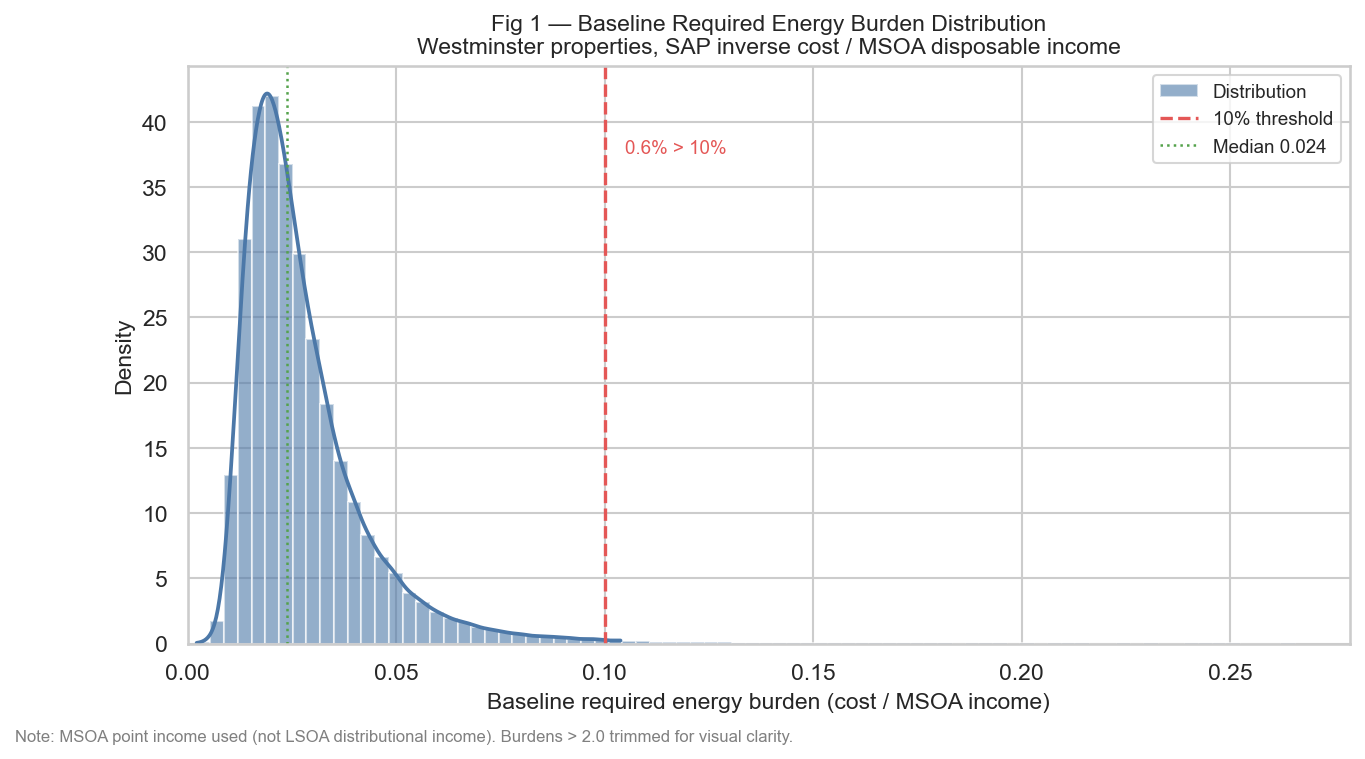
\includegraphics[width=\linewidth]{paper/figures/baseline_required_energy_burden_distribution.png}
\caption{Baseline required energy burden distribution for Westminster properties, using SAP-inverse required energy cost divided by MSOA disposable income. The figure shows the current-price point-income burden metric; it is a baseline affordability measure, not a future fuel-price-shock result.}
\label{fig:baseline-burden-distribution}
\end{figure}

Figure~\ref{fig:burden-prob-distribution} reports the distributional counterpart: the probability that required energy burden exceeds 10 percent when local LSOA income distributions are used. Its median is 0.0525, and the top-decile threshold used for the HR\_TOP10 burden-probability group is 0.311. The contrast between Figures~\ref{fig:baseline-burden-distribution} and \ref{fig:burden-prob-distribution} is substantively important. It shows why Westminster exposure cannot be inferred from a single area-income point estimate: the point burden is usually low, while the income-tail probability has a much wider distribution.

\begin{figure}[H]
\centering
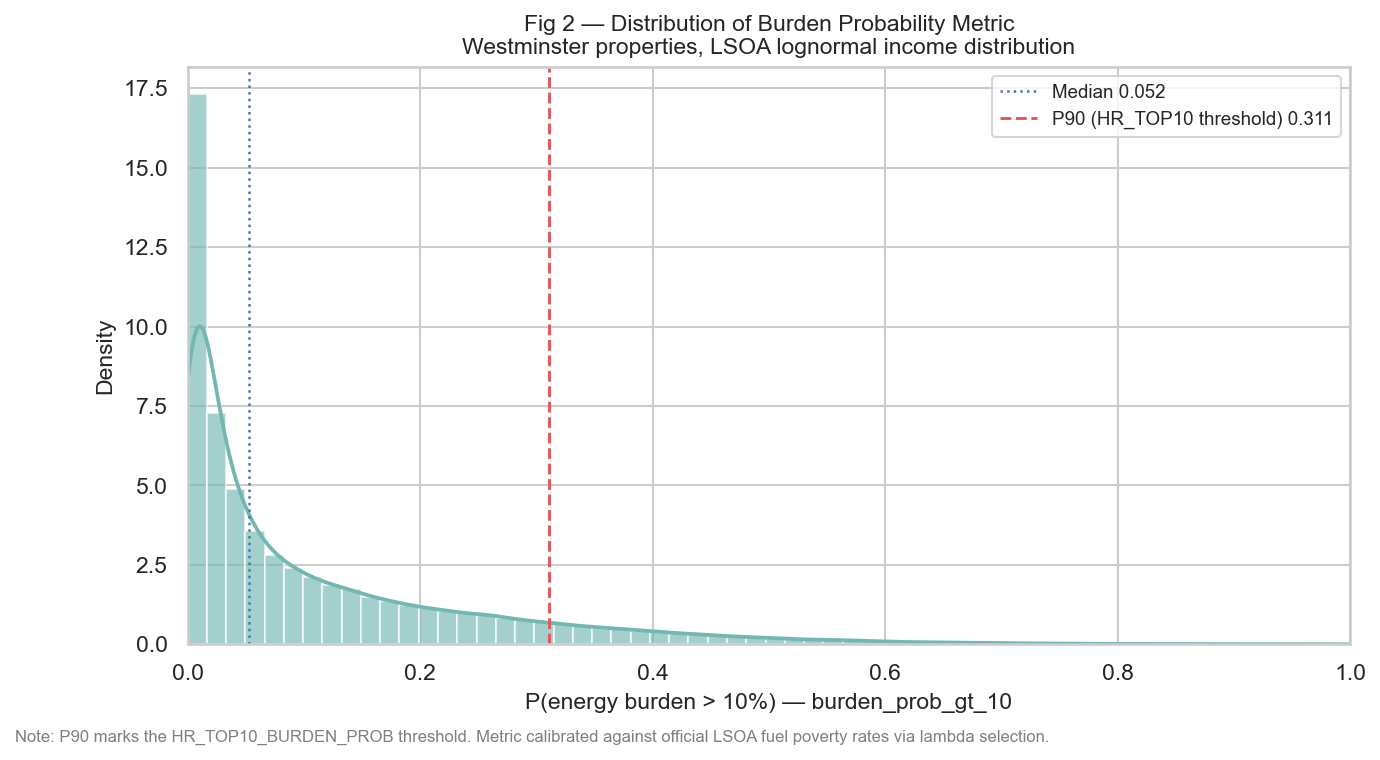
\includegraphics[width=\linewidth]{paper/figures/baseline_burden_probability_distribution.png}
\caption{Distribution of the baseline burden-probability metric, \texttt{burden\_prob\_gt\_10}. The metric uses constrained LSOA lognormal income distributions to estimate the probability that required energy burden exceeds 10 percent. It identifies current income-tail exposure and does not yet include price-shock scenarios.}
\label{fig:burden-prob-distribution}
\end{figure}

The extract also clarifies the housing and fuel composition of the current high-burden tail. Figure~\ref{fig:baseline-high-burden-property-type} shows that flats dominate Westminster's overall stock, but houses and maisonettes are overrepresented in high-burden groups relative to their stock share. Figure~\ref{fig:baseline-high-burden-main-fuel} shows that gas dominates all groups because it dominates the stock, while electricity's share rises slightly in the HR groups. These figures support a layered interpretation: current burden exposure is produced by stock composition, property type, required demand, income distribution, and fuel exposure together, not by one variable alone.

\begin{figure}[H]
\centering
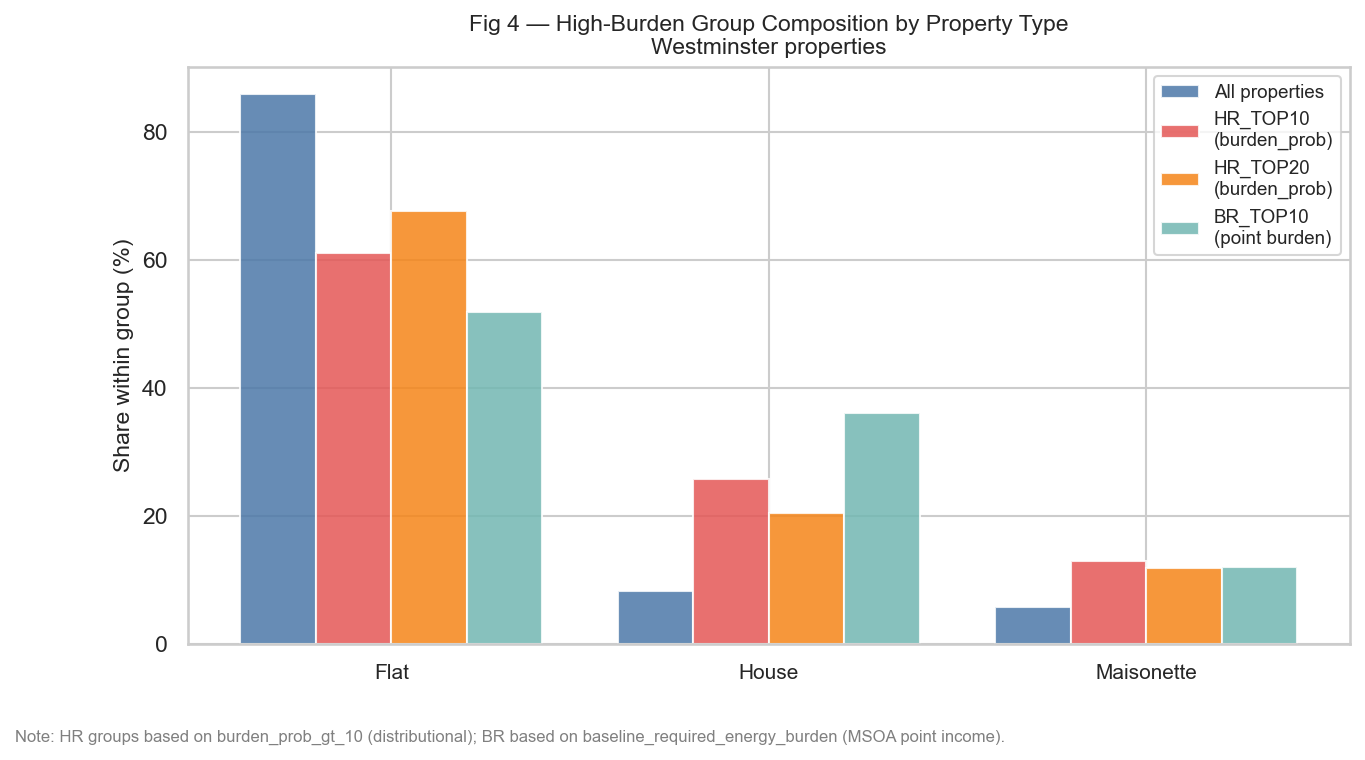
\includegraphics[width=\linewidth]{paper/figures/baseline_high_burden_by_property_type.png}
\caption{Composition of baseline high-burden groups by property type. HR groups are based on \texttt{burden\_prob\_gt\_10}; BR groups are based on deterministic baseline required energy burden using MSOA point income.}
\label{fig:baseline-high-burden-property-type}
\end{figure}

\begin{figure}[H]
\centering
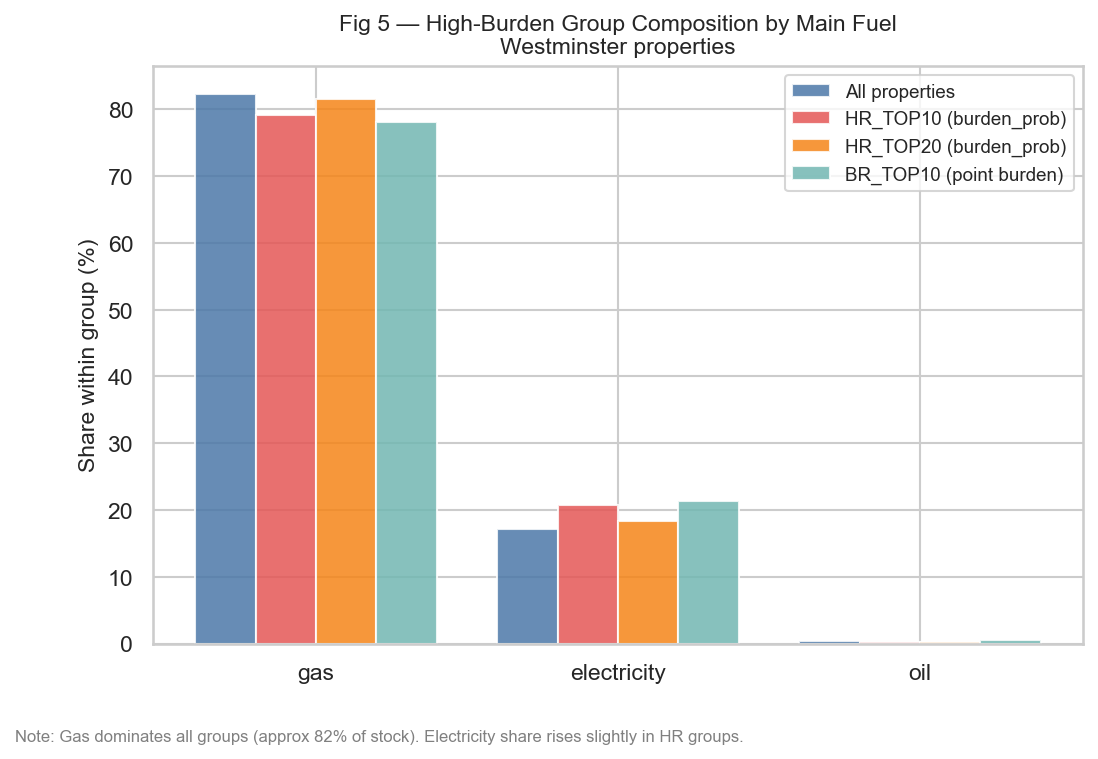
\includegraphics[width=0.86\linewidth]{paper/figures/baseline_high_burden_by_main_fuel.png}
\caption{Composition of baseline high-burden groups by main fuel. The figure shows gas dominance in the stock and a modest overrepresentation of electricity in the HR groups; it motivates fuel-specific price-shock modelling rather than claims about completed fuel price risk.}
\label{fig:baseline-high-burden-main-fuel}
\end{figure}

Third, the baseline module generates a modelled LSOA fuel-poverty comparison used for calibration diagnostics. The latest sensitivity run has a mean modelled-minus-official LSOA fuel-poverty-rate error of -0.0174 and a worst absolute error of 0.133 under the central income-anchor scenario. Weighted MSOA-level RMSE is similar across the central, upper-confidence-limit, and lower-confidence-limit scenarios, with means of 0.04944, 0.05022, and 0.04821 respectively. This residual gap is substantively useful rather than merely technical: it shows that income-tail matching alone does not reproduce official fuel-poverty geography, reinforcing the paper's distinction between income deprivation, required energy burden, dwelling fabric, heating systems, tenure, and future price risk.

Figures~\ref{fig:lsoa-income-pdf-scenarios-1}--\ref{fig:lsoa-income-pdf-scenarios-3} report the promoted LSOA income PDF scenario panels from the May 2026 read-only sensitivity run. They should be read as sensitivity diagnostics for the synthetic income layer. The solid, dashed, and dotted curves compare central, upper-confidence-limit, and lower-confidence-limit MSOA income anchors while holding the lower-tail constraint and required-energy-cost logic fixed. The red vertical marker is the \pounds 19{,}009 income-tail threshold used in the current module. These figures therefore support the baseline burden model by showing how local lower-tail assumptions vary across LSOAs and MSOAs; they do not yet measure future household fuel price risk.

\begin{figure}[H]
\centering
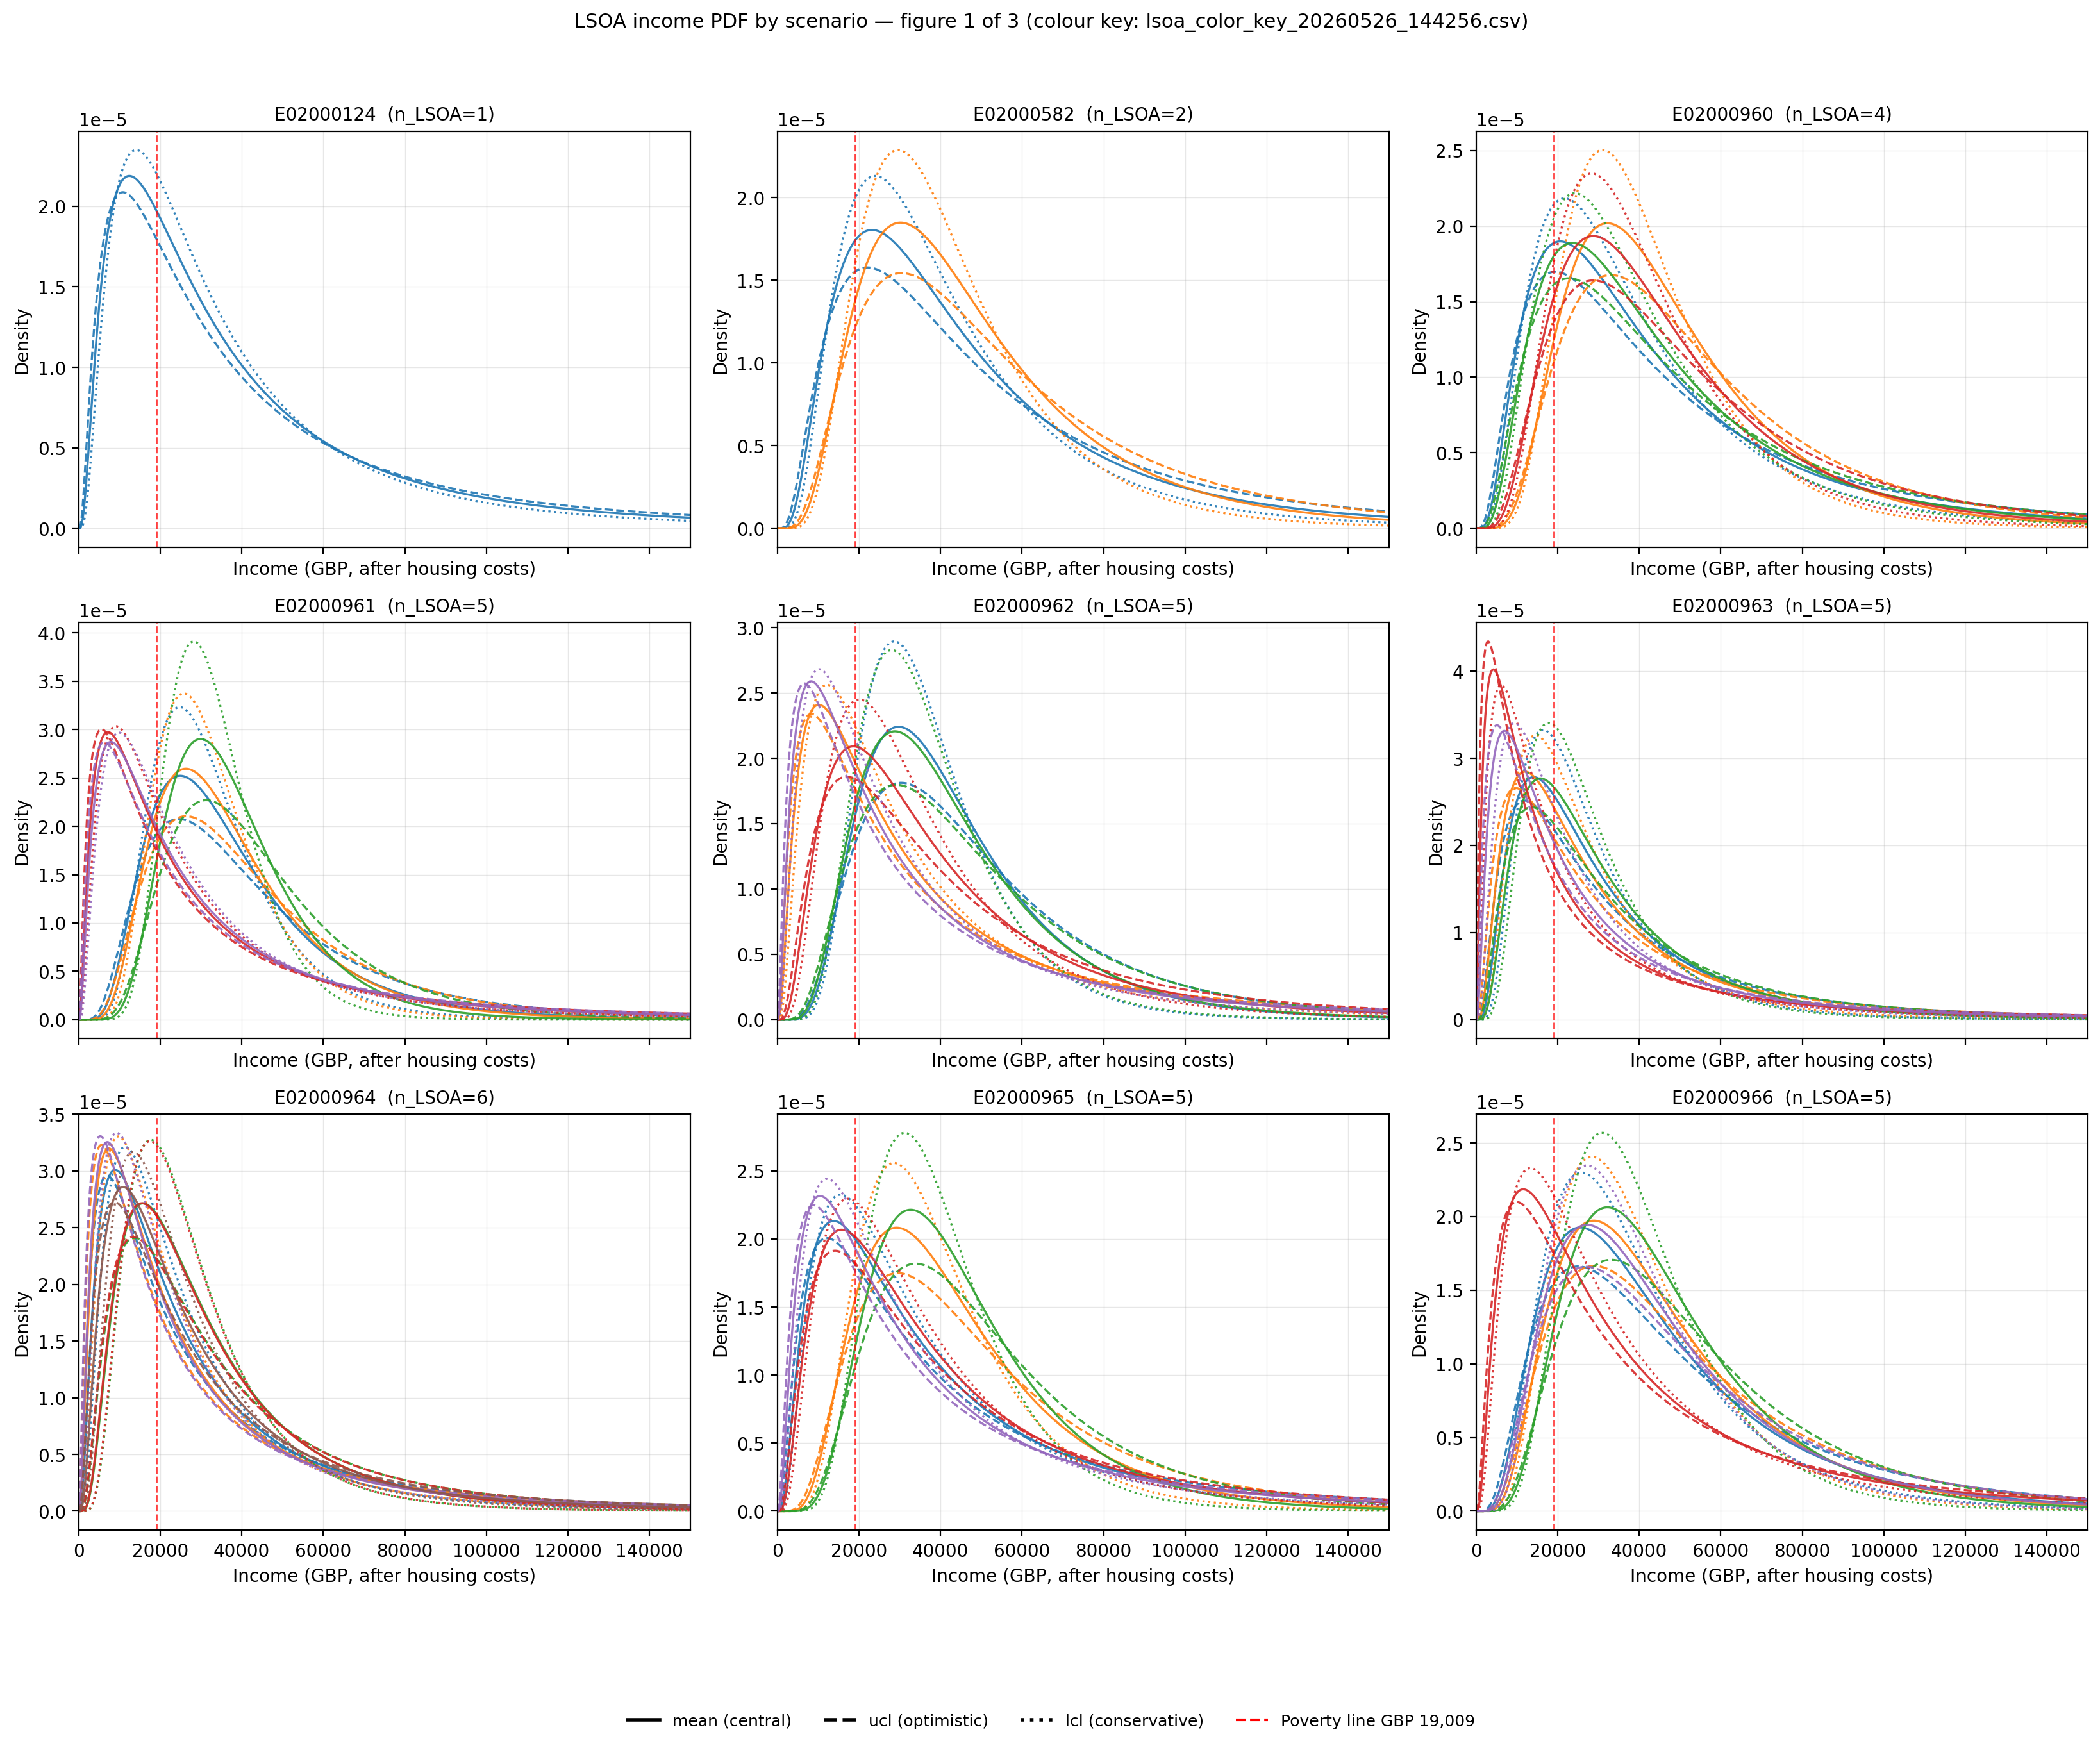
\includegraphics[width=\linewidth]{paper/figures/baseline_income_pdf_scenarios_1.png}
\caption{LSOA income PDF scenario sensitivity, panel set 1 of 3. The curves compare central, upper-confidence-limit, and lower-confidence-limit MSOA after-housing-cost income anchors for constrained synthetic LSOA income distributions; the red line marks the \pounds 19{,}009 lower-tail threshold.}
\label{fig:lsoa-income-pdf-scenarios-1}
\end{figure}

\begin{figure}[H]
\centering
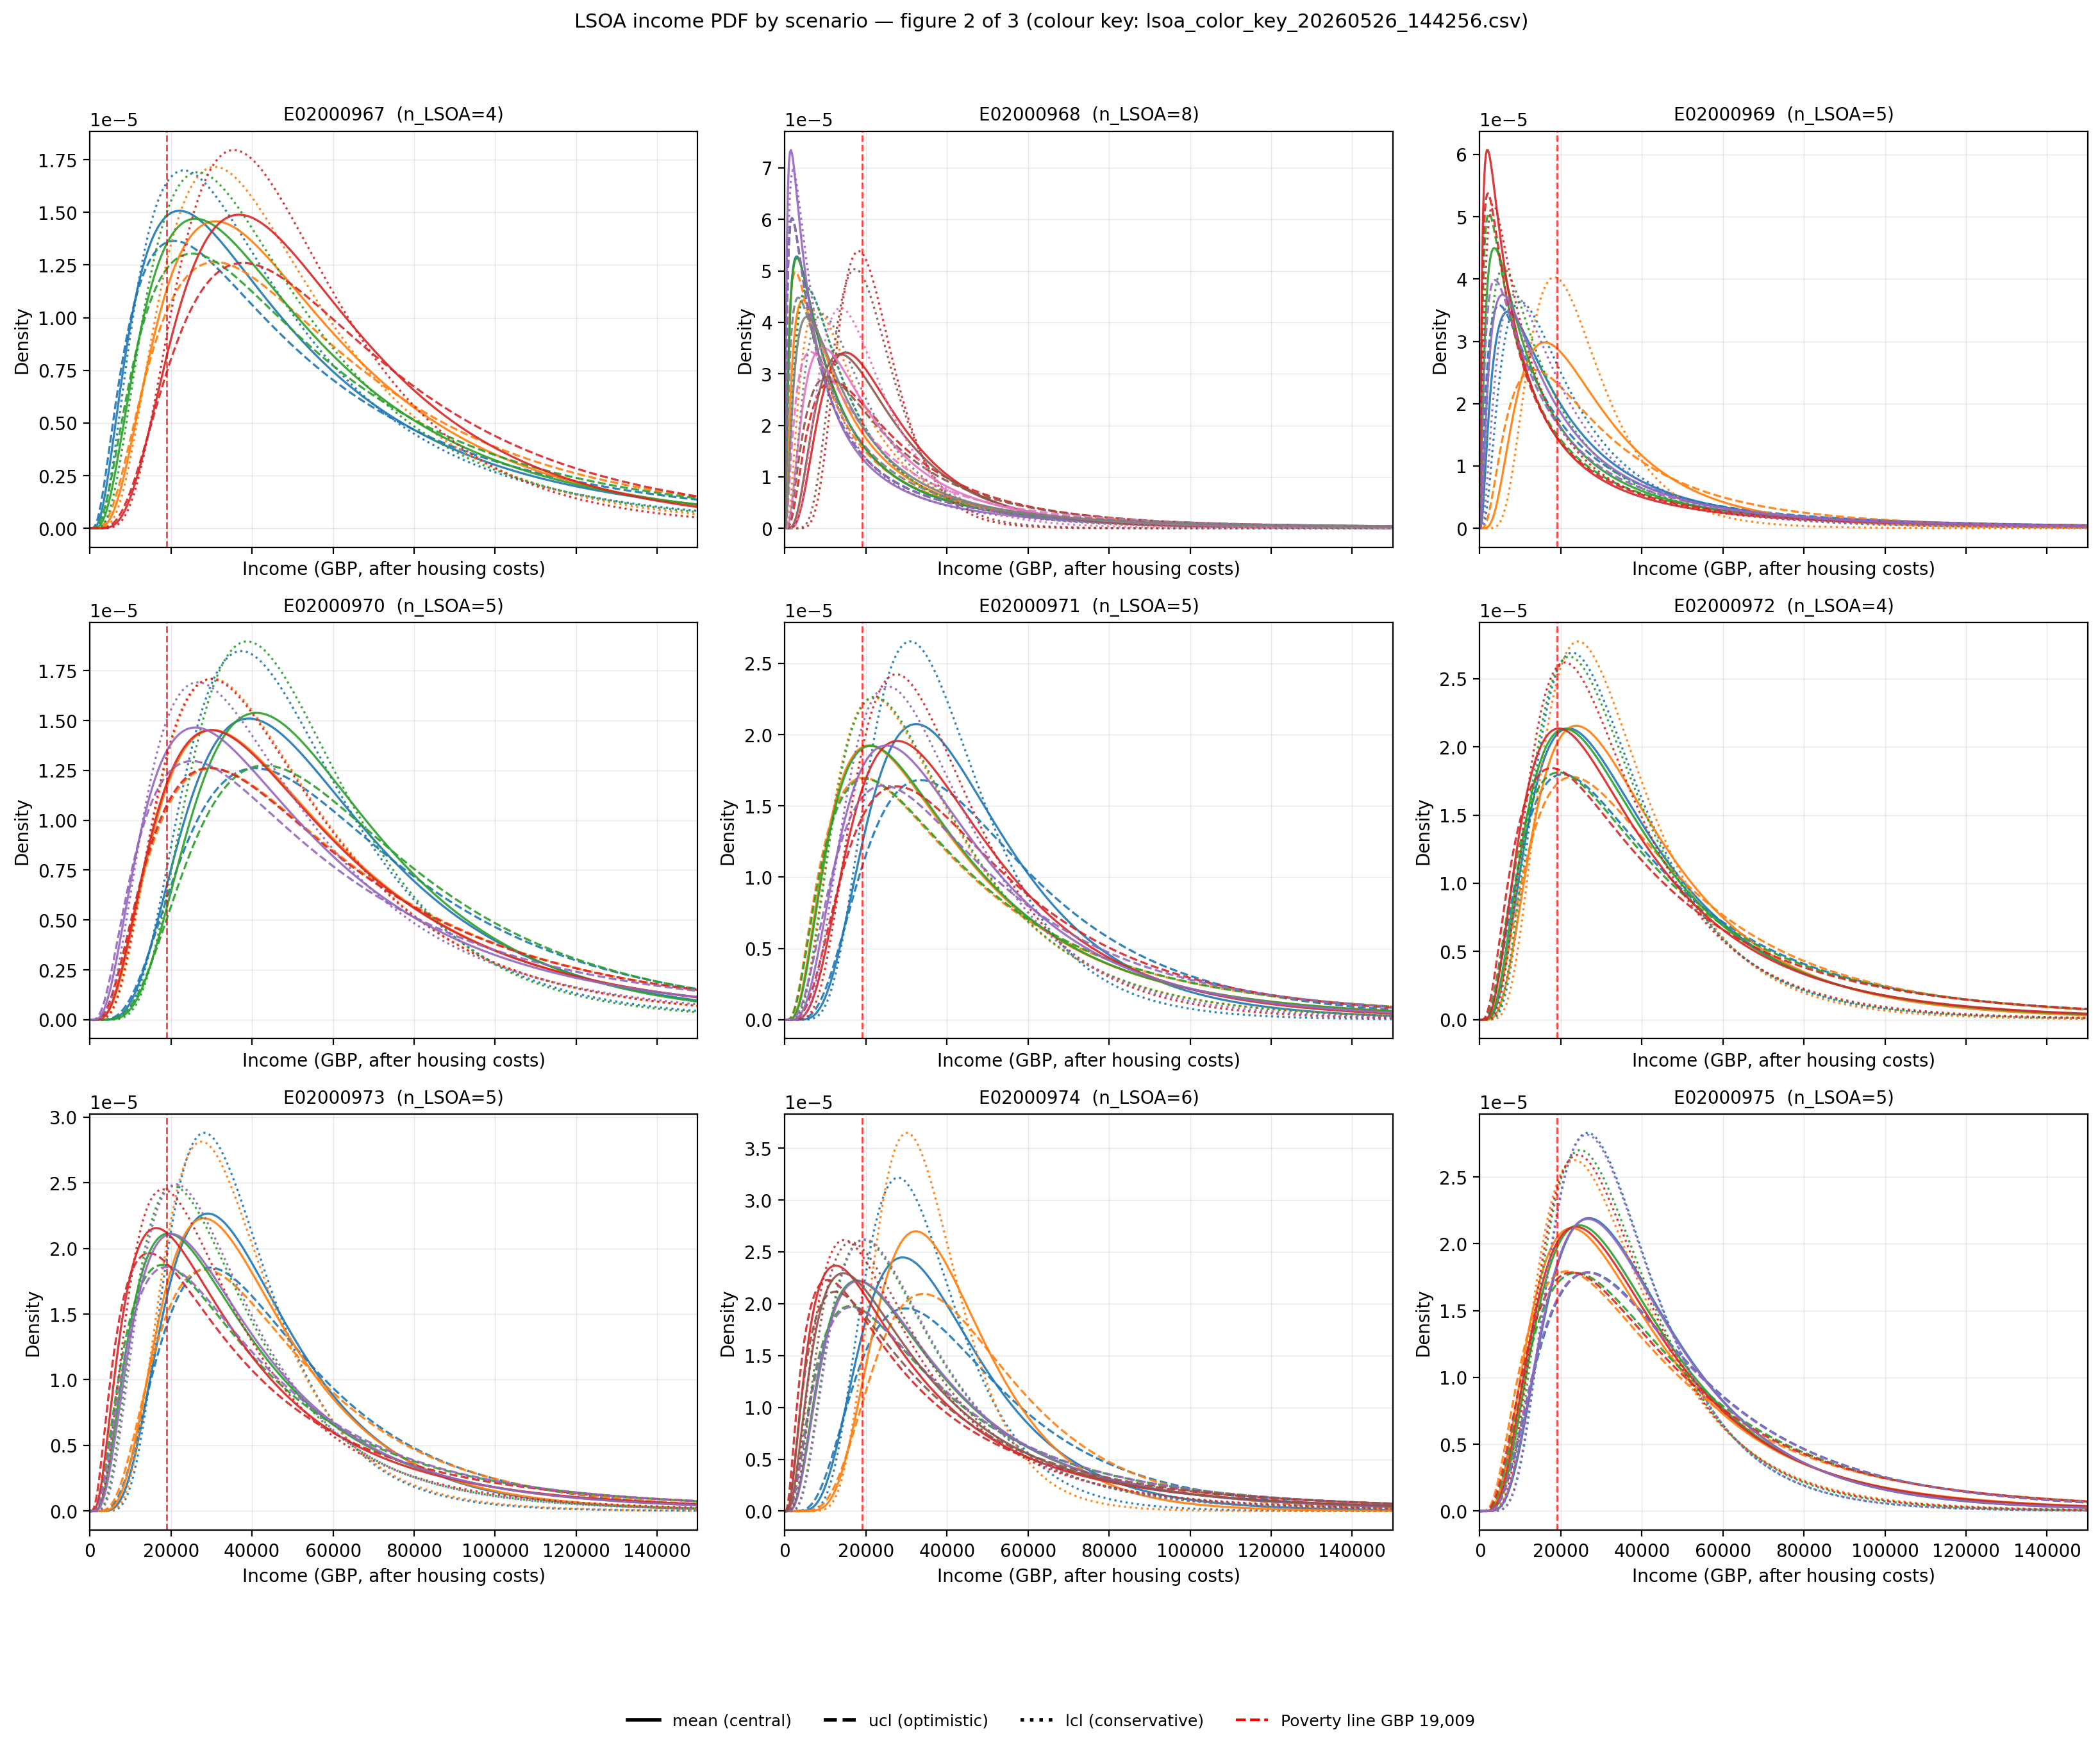
\includegraphics[width=\linewidth]{paper/figures/baseline_income_pdf_scenarios_2.png}
\caption{LSOA income PDF scenario sensitivity, panel set 2 of 3. The figure continues the diagnostic comparison of income-anchor uncertainty across Westminster MSOAs and should be interpreted as a baseline burden-modelling input rather than an observed household income distribution.}
\label{fig:lsoa-income-pdf-scenarios-2}
\end{figure}

\begin{figure}[H]
\centering
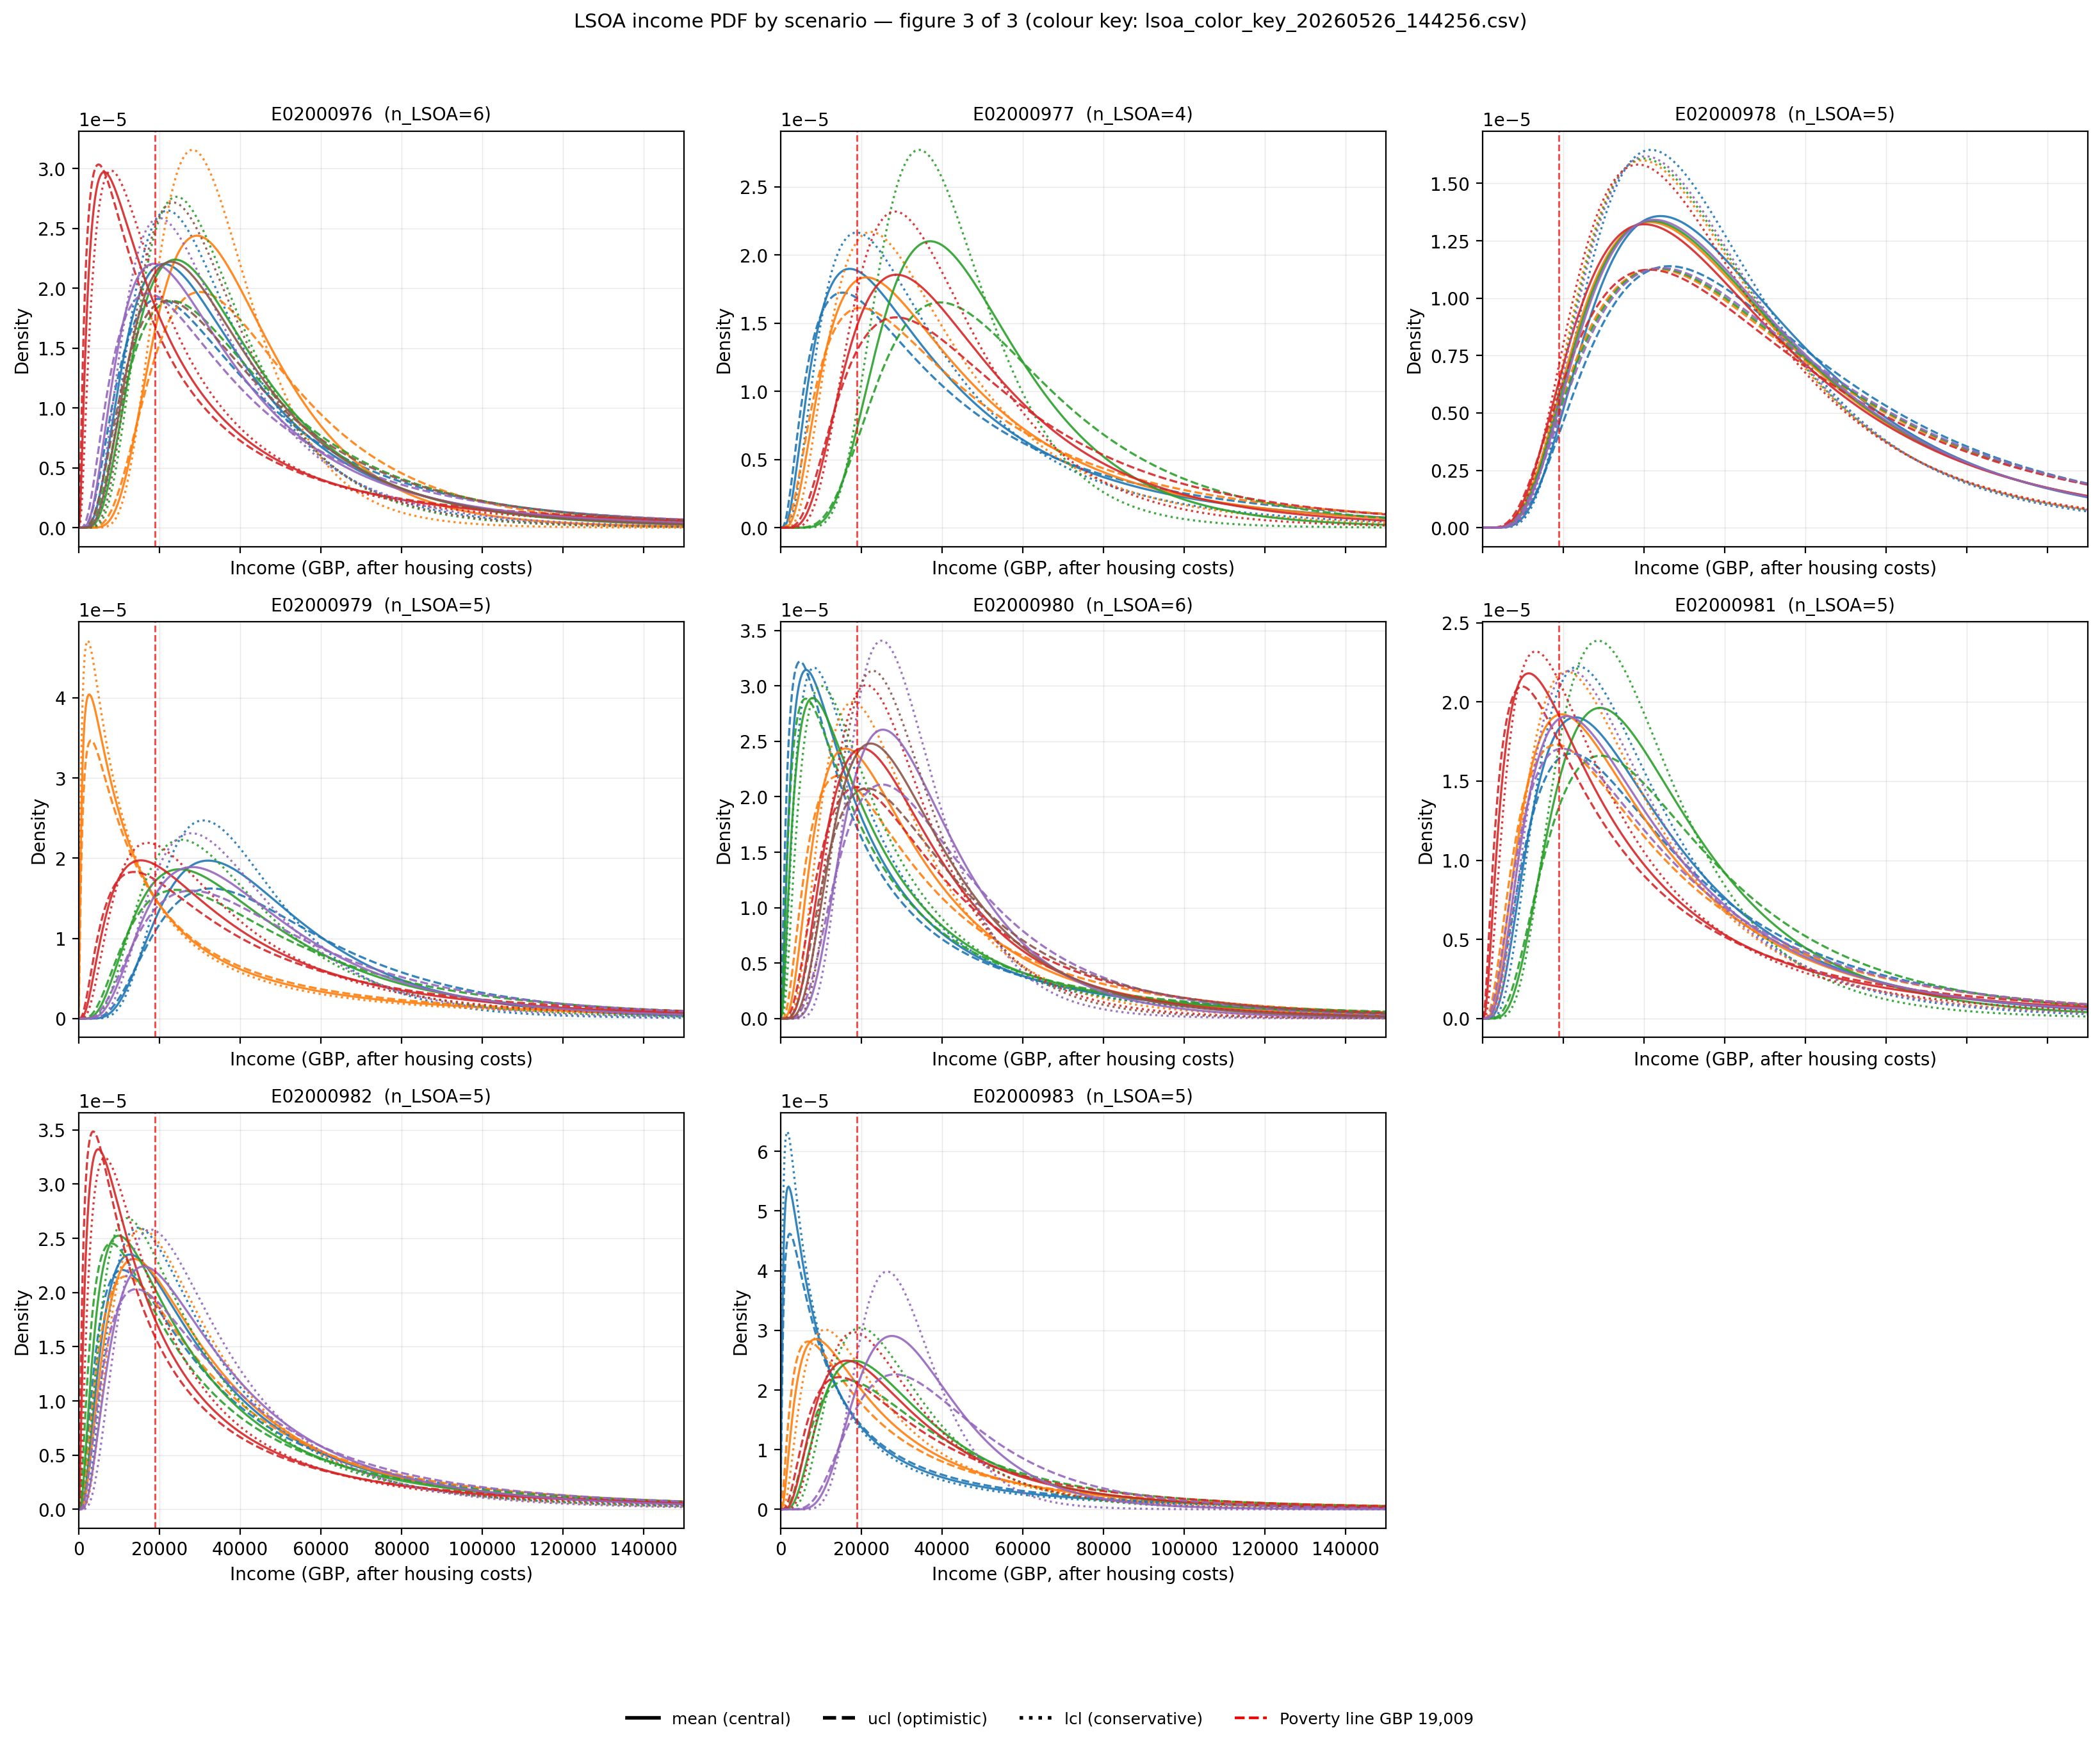
\includegraphics[width=\linewidth]{paper/figures/baseline_income_pdf_scenarios_3.png}
\caption{LSOA income PDF scenario sensitivity, panel set 3 of 3. The panels show that income-anchor uncertainty shifts selected lower-tail distributions, while the residual modelled-versus-official fuel-poverty gap remains a construct-alignment limitation rather than a price-risk result.}
\label{fig:lsoa-income-pdf-scenarios-3}
\end{figure}

\subsection{Implemented Baseline-Cost Sensitivity Outputs}

The energy-cost price-structure sensitivity archive adds a second baseline diagnostic: whether current high-burden rankings depend on the cost definition used before price shocks are introduced. The archive compares SAP-inverse required cost, EPC heating plus hot water plus lighting component cost, an exploratory unit-price-only reconstruction, and a unit-plus-standing reconstruction. It is explicitly a baseline-cost sensitivity exercise, not a final household fuel price risk model.

The main result is that baseline cost definition materially affects current exposure rankings. SAP-inverse cost has a median of \pounds 1,045 per year and a mean of \pounds 1,256 per year, while the EPC component total has a median of \pounds 651 per year and a mean of \pounds 805 per year. The median EPC-component-to-SAP-inverse cost ratio is 0.566, and 89.2 percent of properties have an EPC component cost below the SAP-inverse cost. The two measures remain correlated, with Pearson correlation 0.713 and Spearman correlation 0.763, but the top-decile high-burden groups overlap only partially: the Jaccard overlap is 0.351 for the top 10 percent and 0.449 for the top 20 percent.

Figure~\ref{fig:sap-epc-cost-scatter} visualises this divergence. It should be interpreted as a robustness warning about translating EPC/SAP information into required annual cost. The EPC component measure excludes cooking and other services implicit in the SAP-inverse total-cost measure, so the figure does not prove that one metric is universally superior. It shows that the paper's exposure rankings depend partly on the baseline-cost boundary selected before price-shock scenarios are introduced.

\begin{figure}[H]
\centering
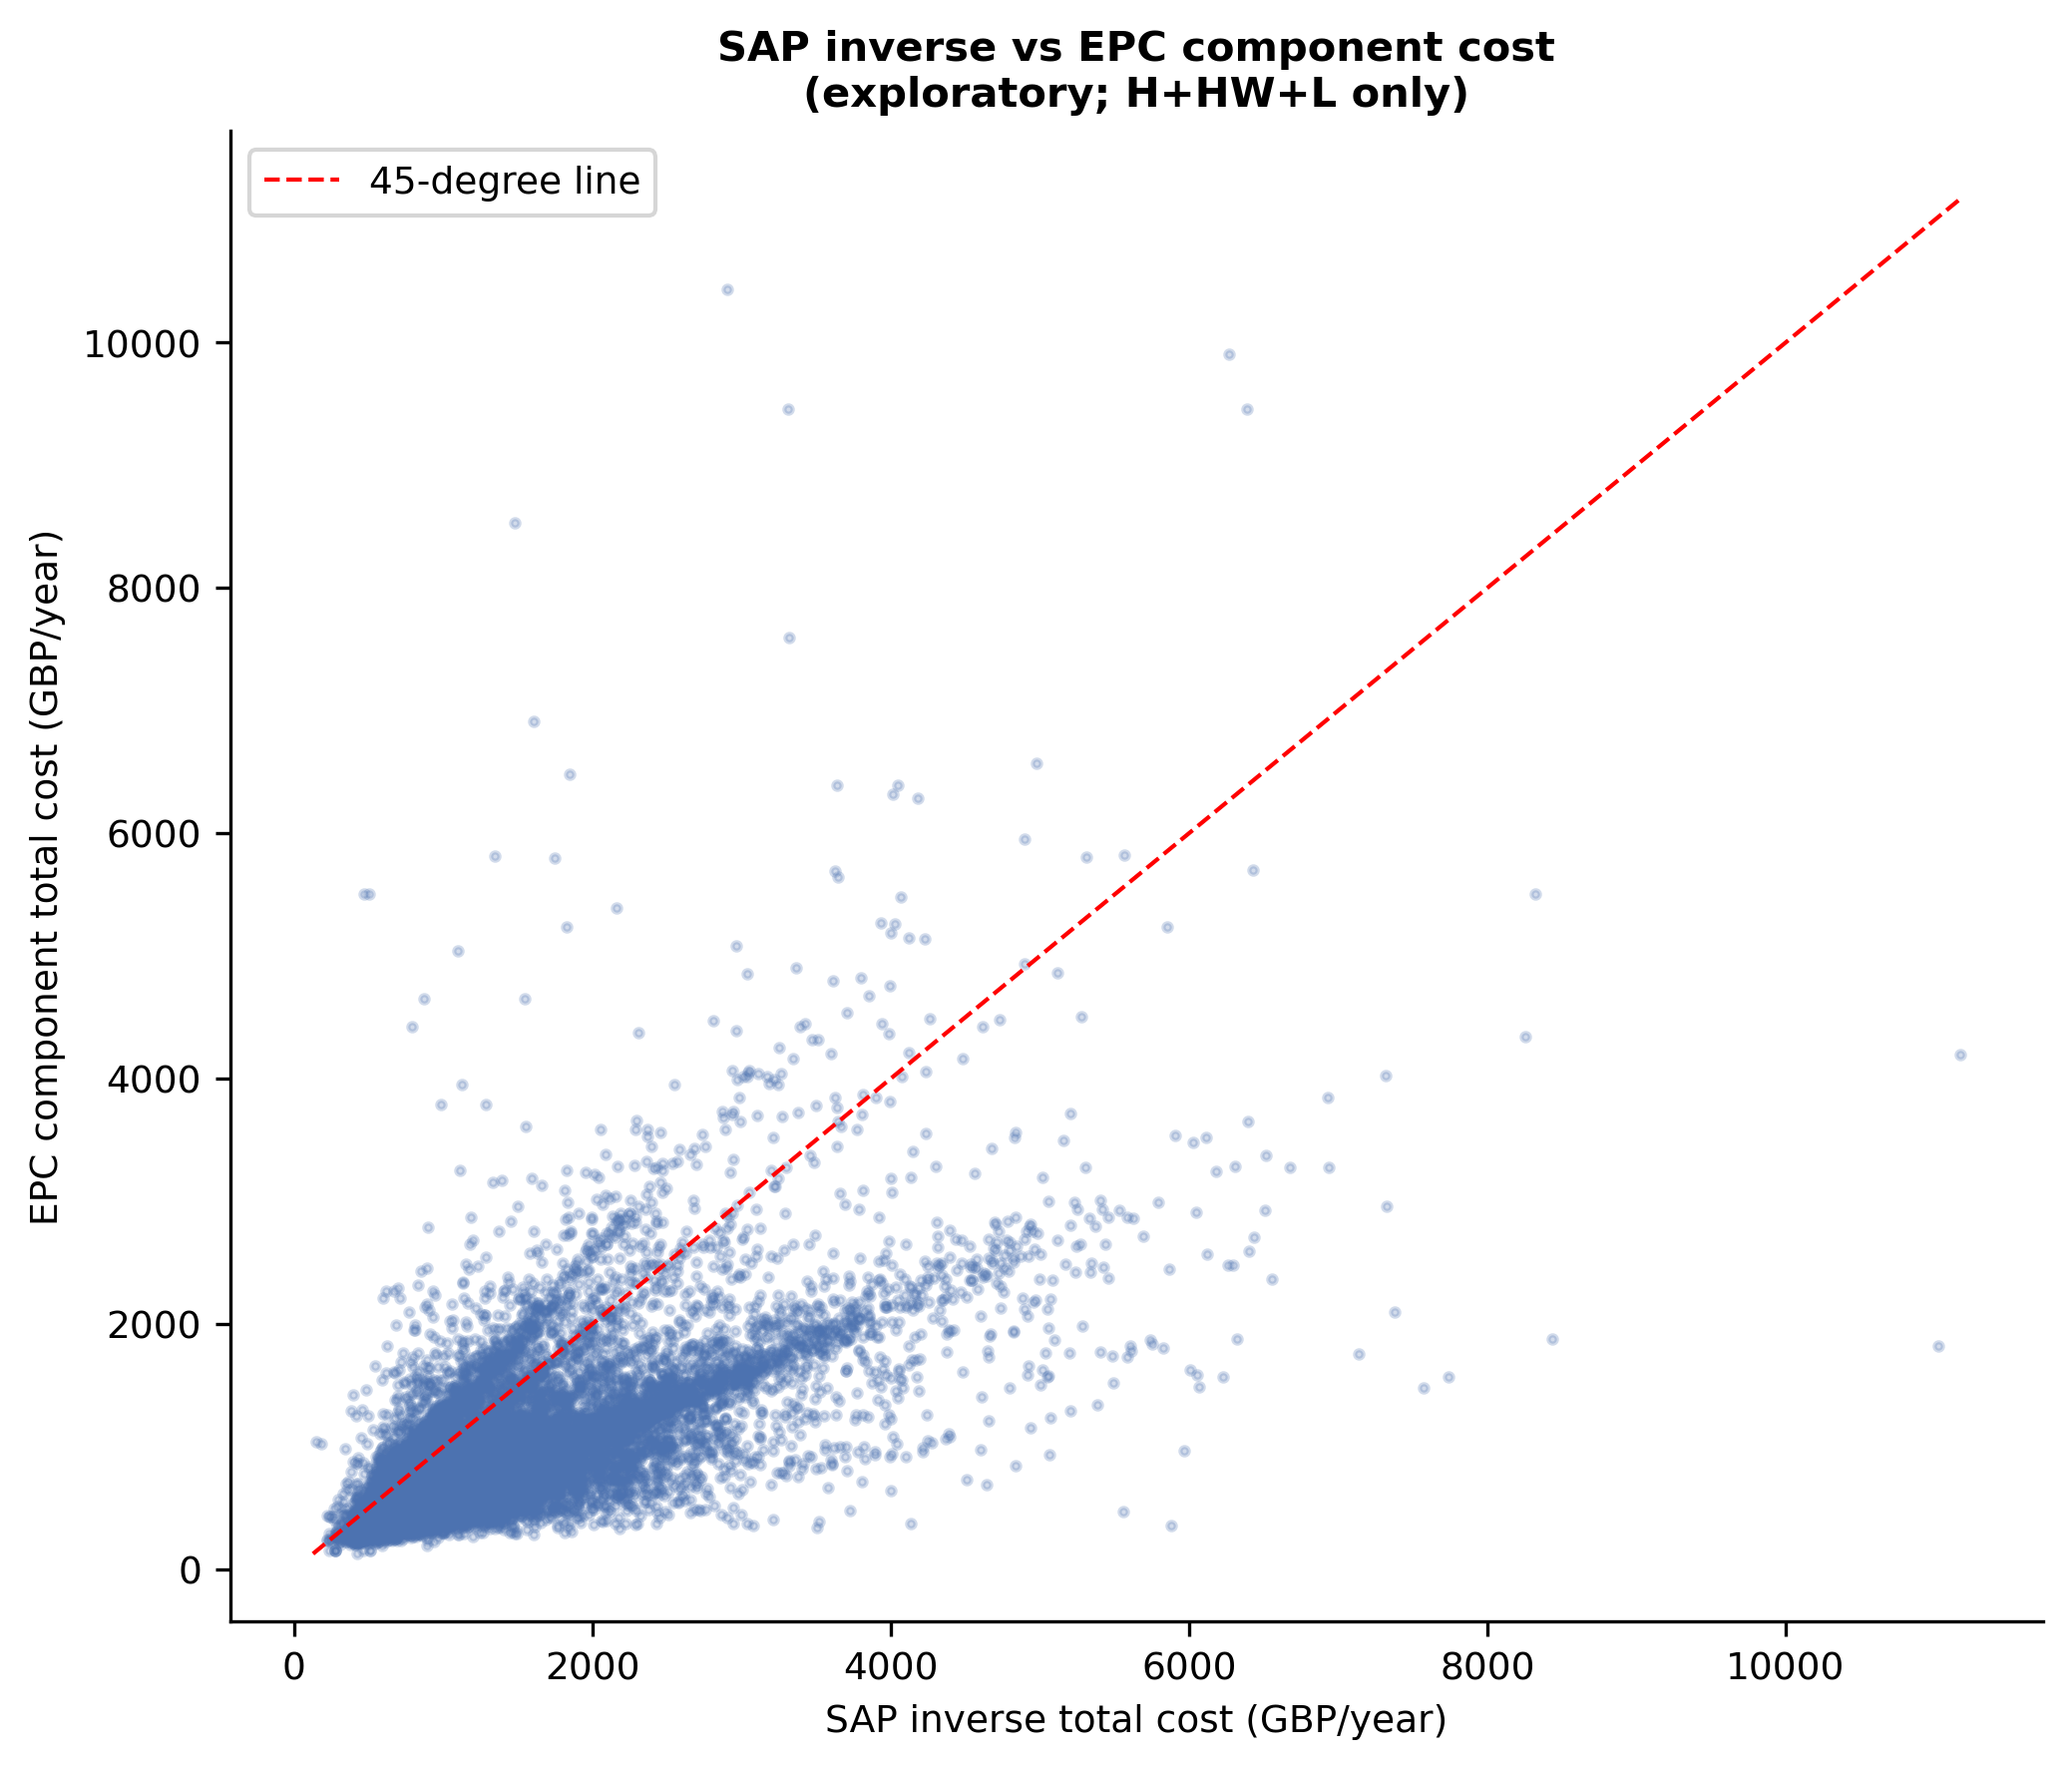
\includegraphics[width=0.88\linewidth]{paper/figures/sap_vs_epc_component_cost_scatter.png}
\caption{SAP-inverse total cost versus EPC heating, hot water, and lighting component cost in the Westminster property-level sample. The scatter shows that alternative translations from EPC/SAP information into required annual cost produce materially different baseline-cost levels and high-burden rankings; the EPC component total excludes cooking and is used here as an exploratory robustness comparator.}
\label{fig:sap-epc-cost-scatter}
\end{figure}

The standing-charge decomposition adds a more specific price-structure diagnostic. Under the current reconstruction, adding standing charges raises burden levels modestly but does not materially reorder the highest-burden decile: the median uplift is about 0.0021 burden units, and the top-decile overlap between the unit-price-only and unit-plus-standing burden measures has a Jaccard value of 0.966. Figure~\ref{fig:standing-burden-uplift-property-type} shows that property-type differentiation in this standing-charge uplift is limited in the current run. This should not be read as evidence that standing charges are unimportant. It means that a full price-shock engine should model standing charges, unit rates, off-peak or dual-tariff structures, electricity/gas price ratios, and policy mitigation separately rather than multiplying a single total-cost scalar.

\begin{figure}[H]
\centering
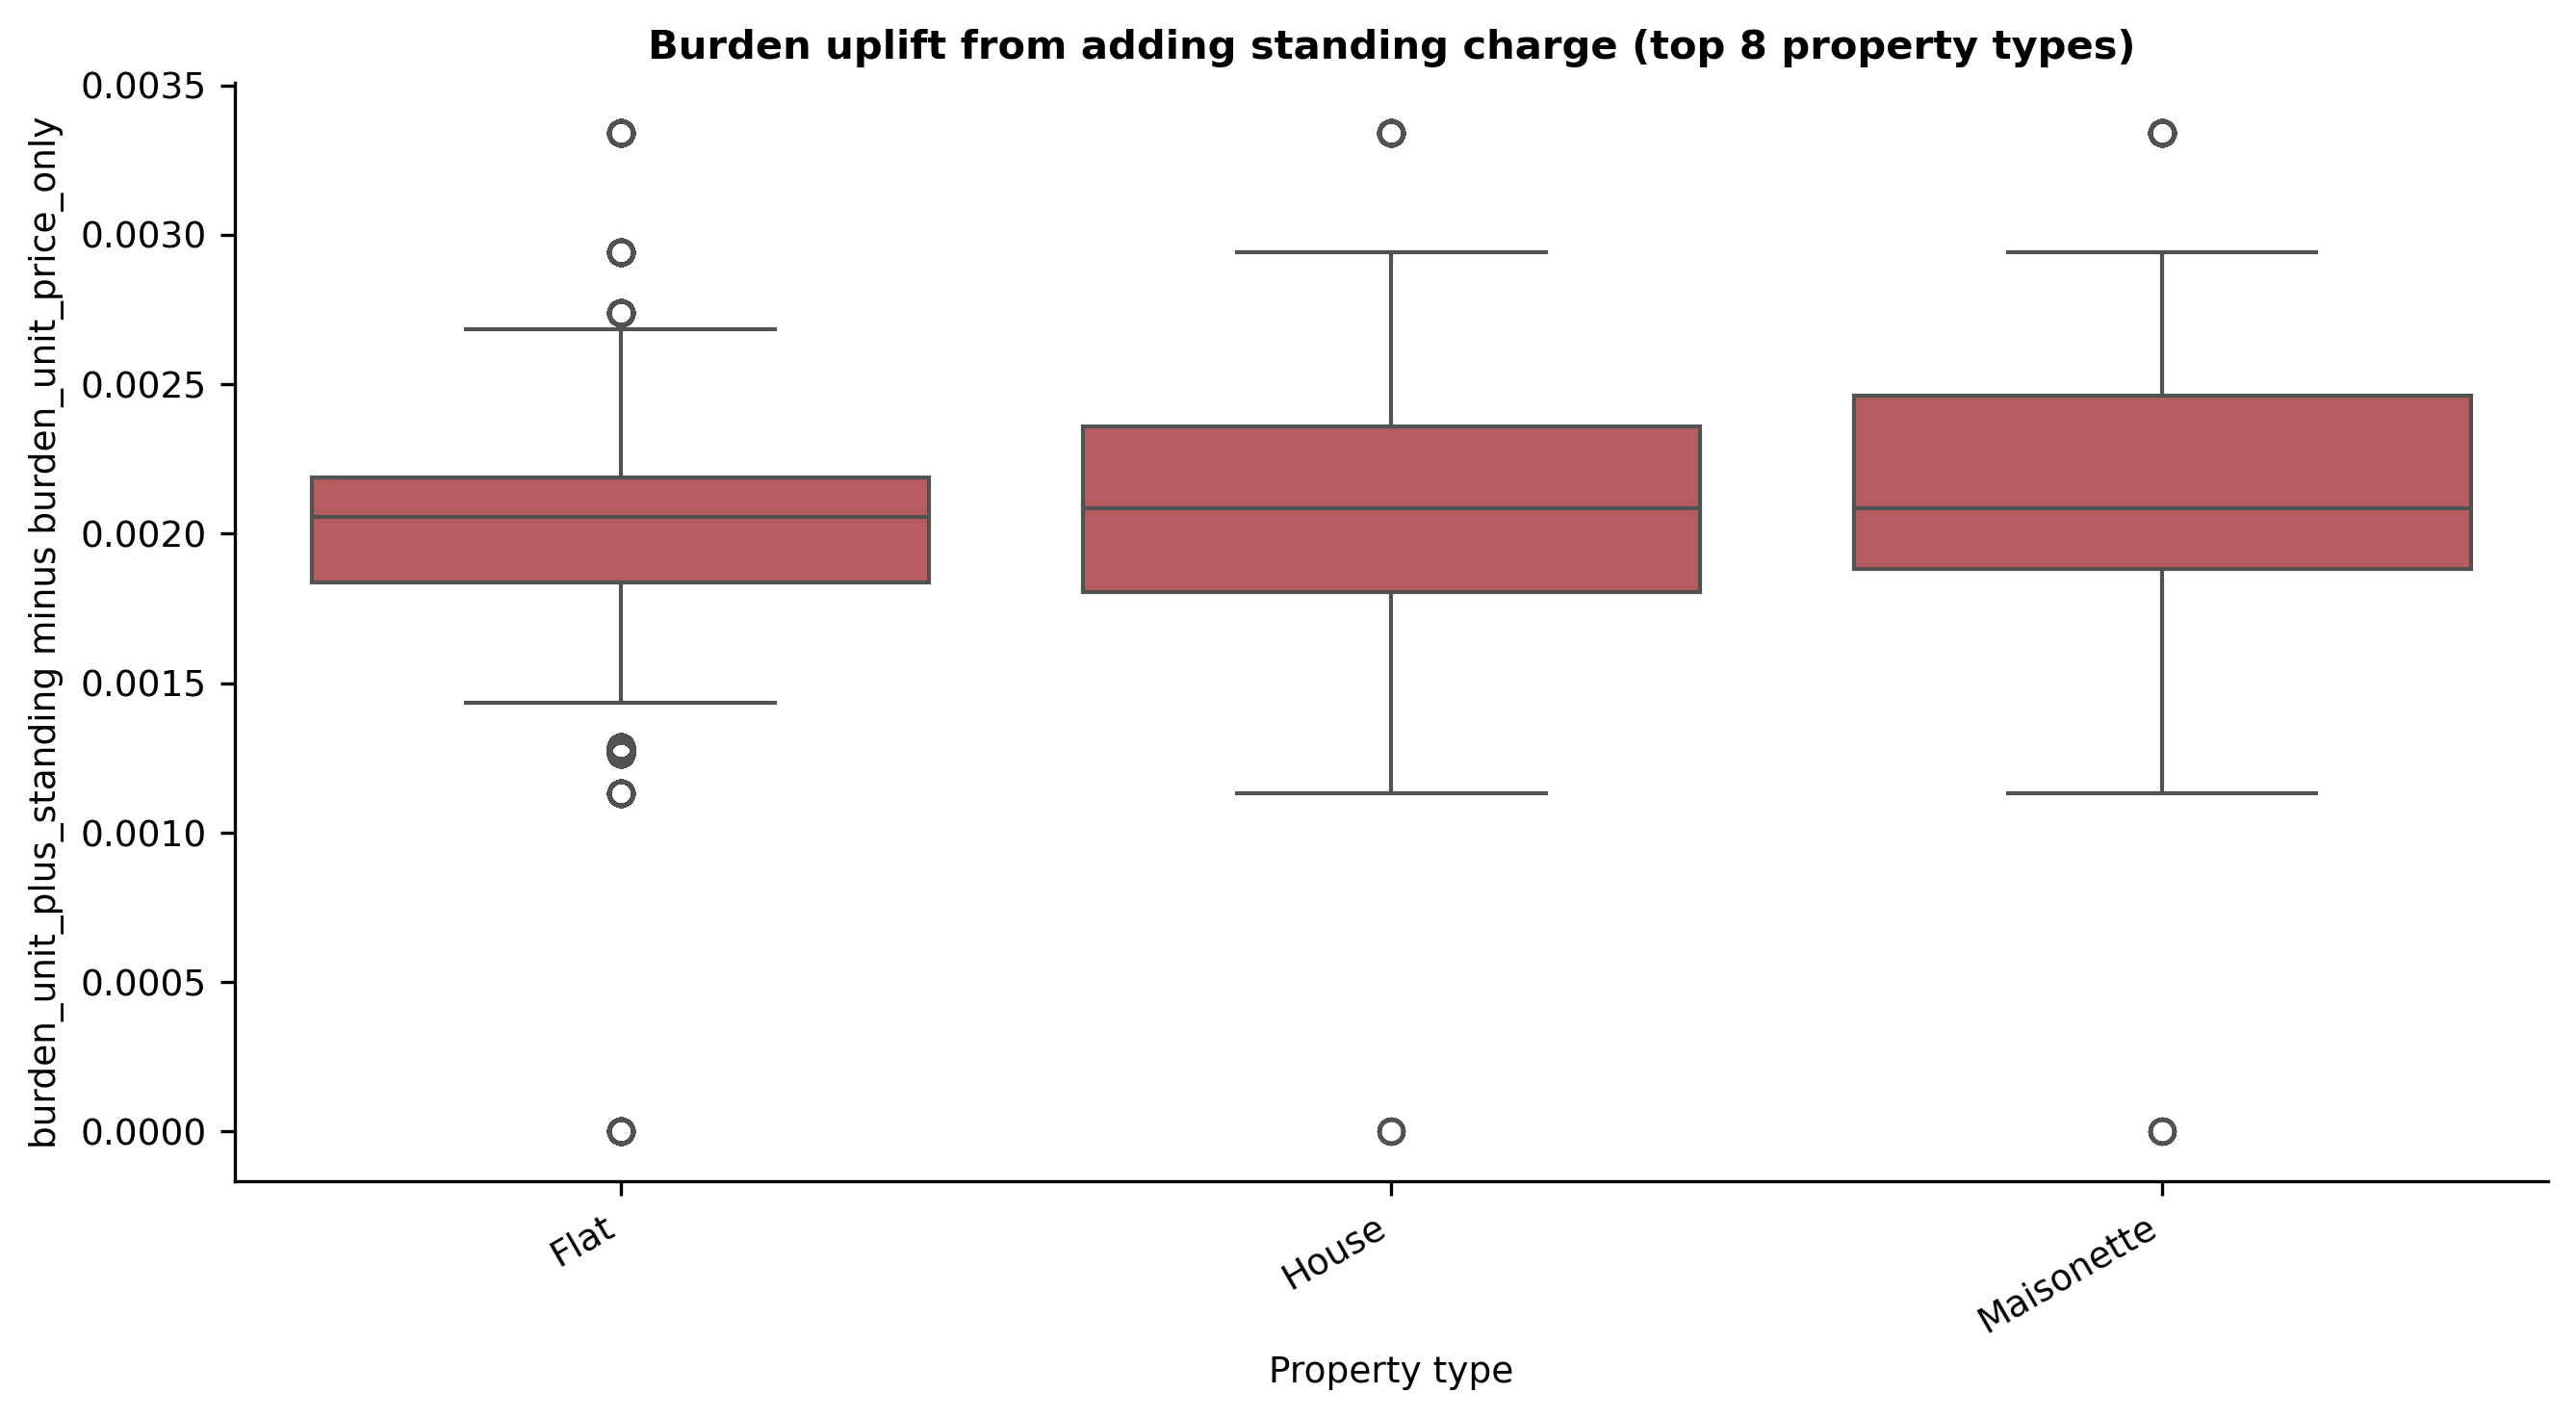
\includegraphics[width=0.82\linewidth]{paper/figures/burden_uplift_from_standing_by_property_type.png}
\caption{Burden uplift associated with adding the standing-charge component by property type. The figure reports an exploratory decomposition using MSOA point income and SAP 10.2 fuel-price mapping; it indicates modest burden-level uplift and limited property-type differentiation in this run, rather than a full standing-charge shock result.}
\label{fig:standing-burden-uplift-property-type}
\end{figure}

\subsection{Implemented High-Risk Explanation Outputs}

The latest high-risk explanation stage adds an audited EPC-enriched stock and a descriptive pathway typology. The enriched master retains 124,980 Westminster property records. After corrected UPRN standardisation, the QA workbook reports a complete match between the master properties and EPC certificate records, with zero unmatched master rows. The corrected EPC tenure proxy distributes the stock into 58,744 private rented properties, 43,686 owner-occupied properties, 20,066 social rented properties, and 2,484 unknown-tenure properties. These tenure categories are analytical proxies and should be interpreted as adaptive-capacity and governance indicators rather than as verified household tenure records.

The implemented high-risk groups remain exploratory and model-based. HR10 contains the 12,500 properties in the top decile of the probability that required energy burden exceeds 10 percent; HR20 contains the 24,996 properties in the top quintile. The deterministic burden robustness groups contain 12,498 BR10 properties and 24,996 BR20 properties, while only 737 properties have a baseline required energy burden above 10 percent under the deterministic baseline measure. As Figure~\ref{fig:hr-br-overlap} shows, HR10 and BR10 overlap for 7,128 properties, or 57.0 percent of each group. This overlap is large enough to show that the probabilistic and deterministic indicators identify a related high-burden tail, but incomplete enough to justify reporting both.

\begin{figure}[H]
\centering
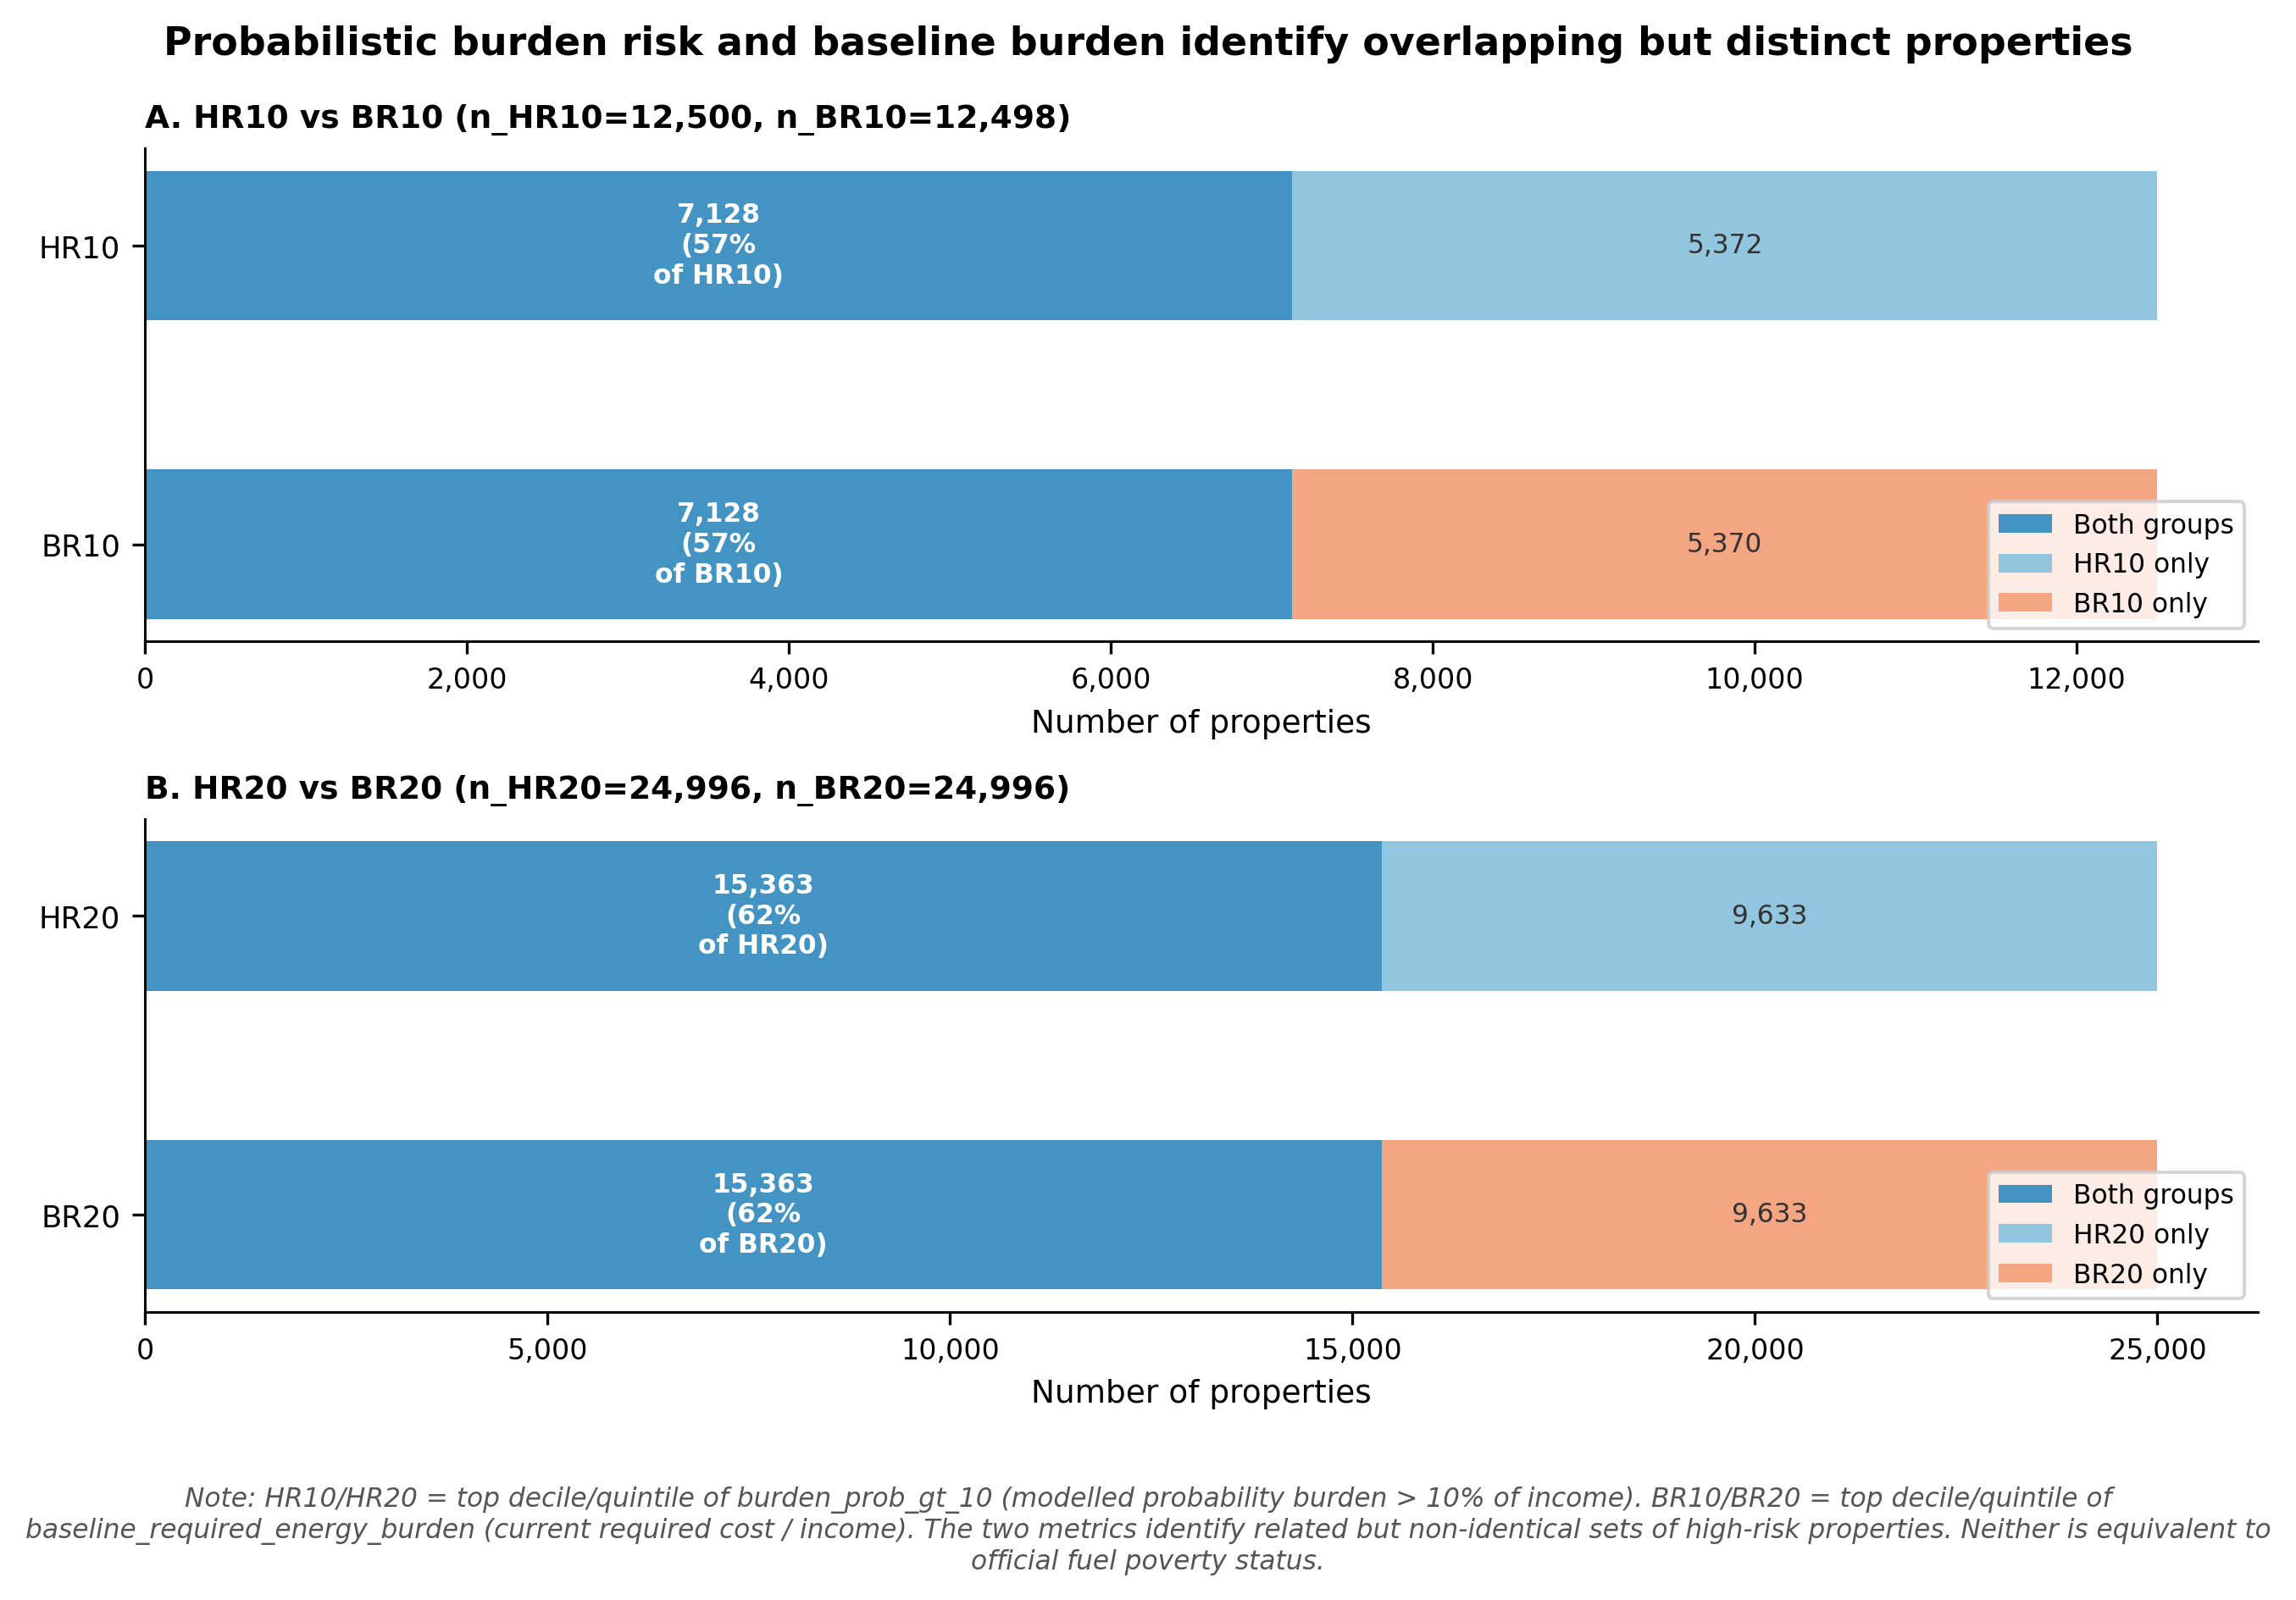
\includegraphics[width=\linewidth]{paper/figures/high_risk_hr_br_overlap.png}
\caption{Overlap between probabilistic high-risk groups (HR10/HR20) and deterministic baseline burden groups (BR10/BR20). The partial overlap shows that income-distribution exposure and deterministic burden intensity identify related but non-identical current high-burden sets.}
\label{fig:hr-br-overlap}
\end{figure}

The strongest descriptive signal in the current outputs is the interaction between dwelling size and energy performance. Figure~\ref{fig:epc-floorarea-hr10} shows that EPC E--F--G properties above 120 m$^2$ have an HR10 share of 69.68 percent and an HR20 share of 85.21 percent, with a median baseline burden of 7.26 percent. E--F--G houses also show high within-type exposure, with an HR10 share of 56.08 percent. By contrast, E--F--G flats have a lower within-type HR10 share of 19.38 percent, but remain important because flats are numerous in the Westminster stock.

\begin{figure}[H]
\centering
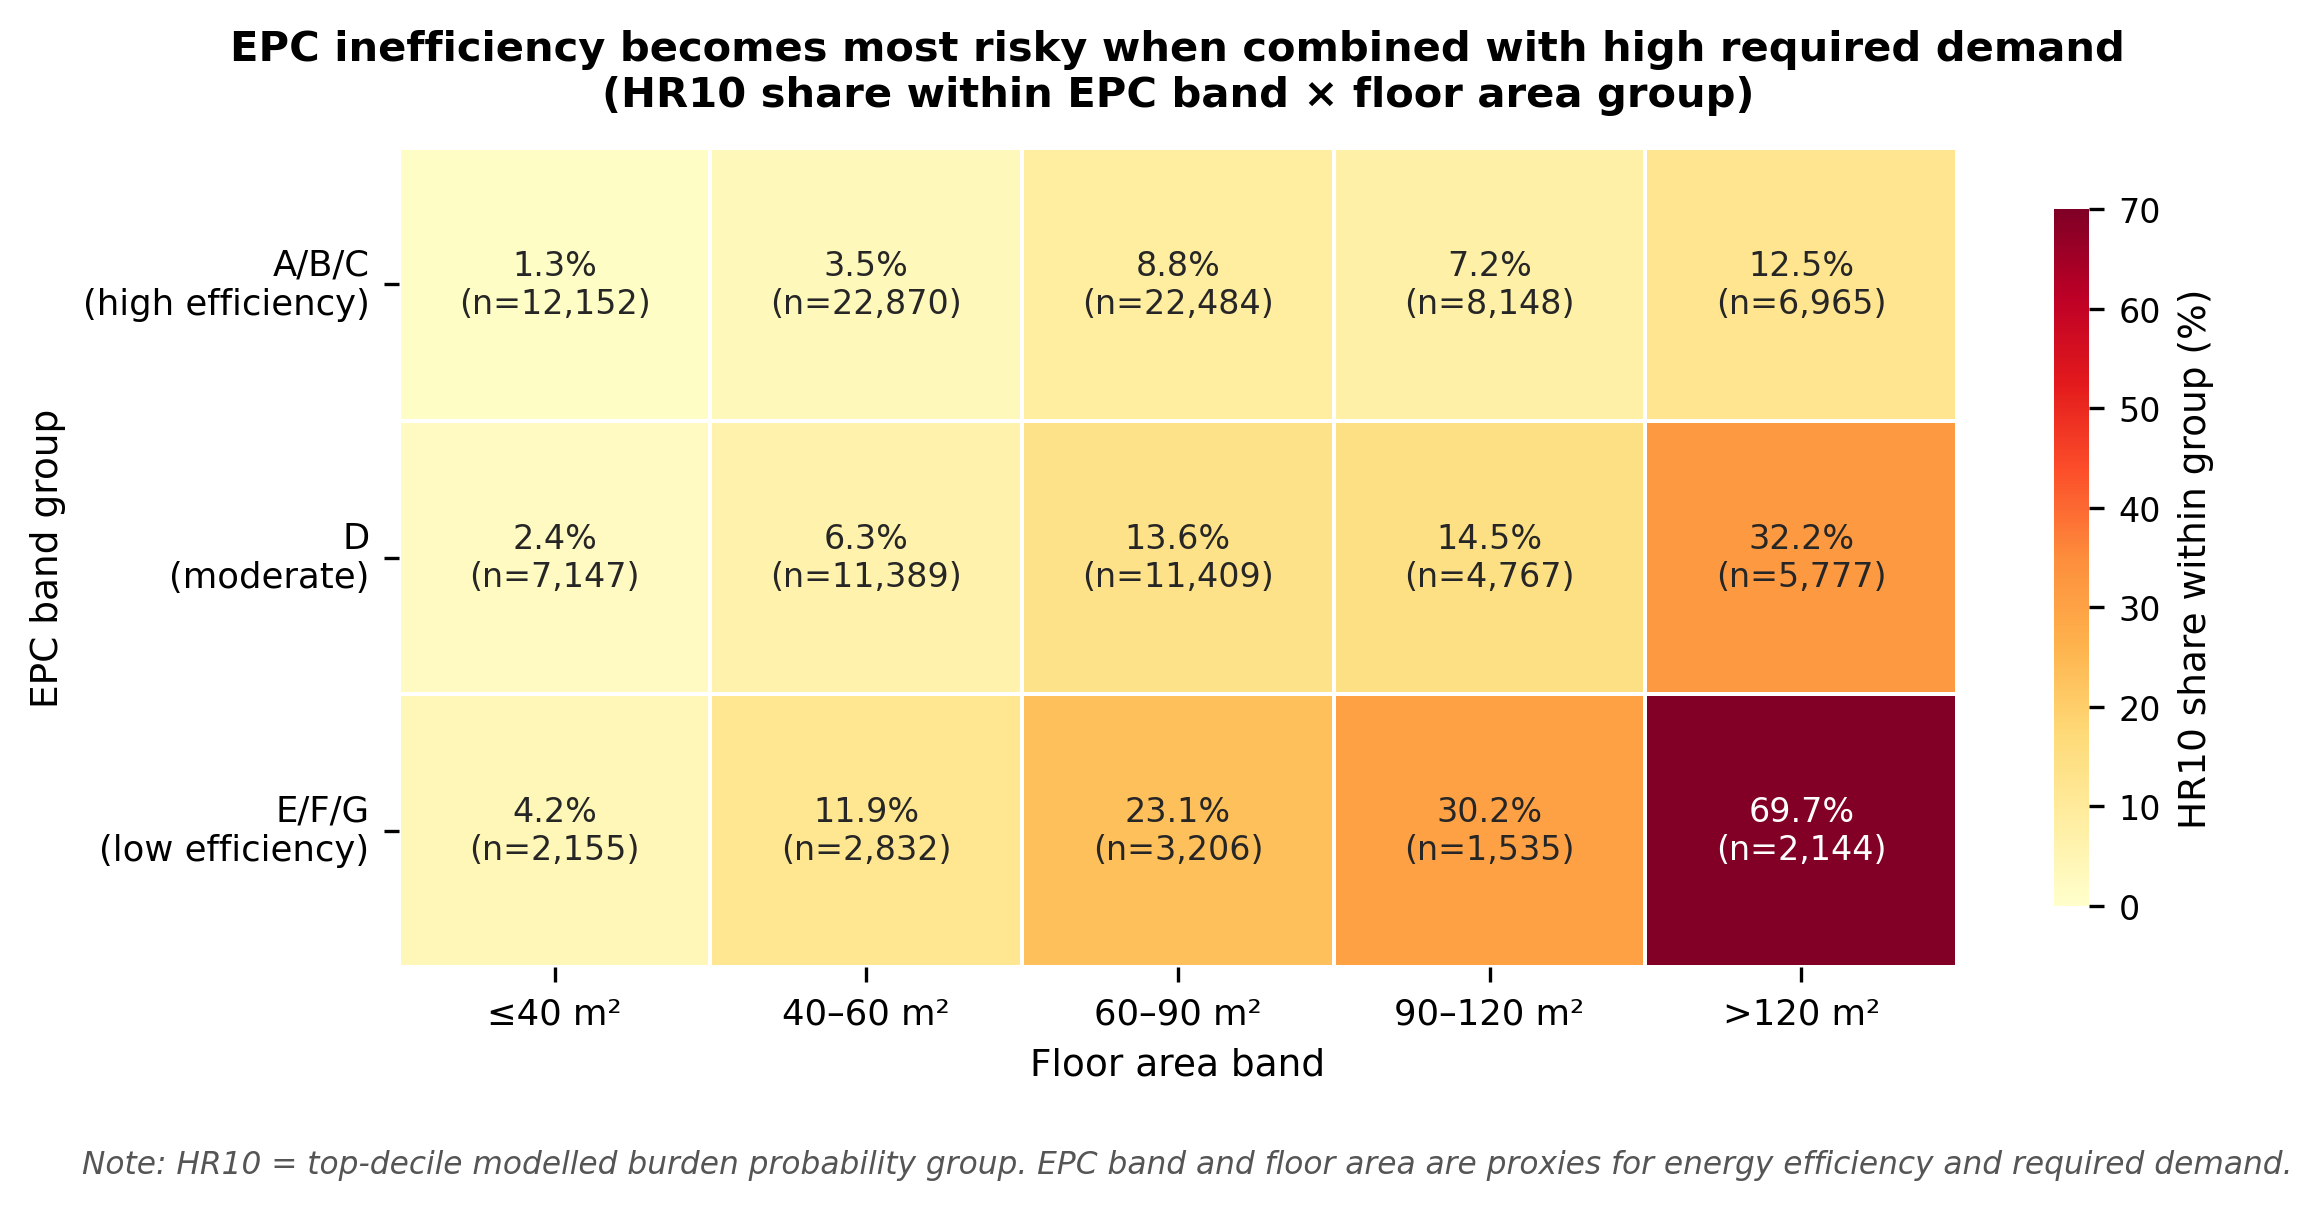
\includegraphics[width=0.86\linewidth]{paper/figures/high_risk_epc_floorarea_heatmap.png}
\caption{HR10 share by EPC band and floor-area group. The heatmap shows that low energy performance becomes most consequential where required demand is amplified by dwelling size; EPC band alone is therefore an incomplete risk signal.}
\label{fig:epc-floorarea-hr10}
\end{figure}

\begin{table}[htbp]
\centering
\footnotesize
\setlength{\tabcolsep}{3pt}
\caption{Current high-risk pathway typology from the latest explanatory run}
\label{tab:high-risk-pathways}
\begin{tabular}{>{\raggedright\arraybackslash}p{0.36\linewidth}rrrr}
\toprule
Pathway & Properties & Stock & HR10 & HR10 contrib. \\
\midrule
Inefficient large owner-occupied gas houses & 2,802 & 2.24\% & 50.25\% & 11.26\% \\
Social rented estate/block risk & 7,016 & 5.61\% & 22.66\% & 12.72\% \\
Private rented weak-fabric gas flats & 34,672 & 27.74\% & 4.18\% & 11.60\% \\
Electric-heated inefficient flats/maisonettes & 10,256 & 8.21\% & 13.83\% & 11.34\% \\
High-demand inefficient maisonettes & 2,220 & 1.78\% & 25.81\% & 4.58\% \\
Other high-risk residual group & 13,063 & 10.45\% & 46.40\% & 48.49\% \\
Not high risk / comparison stock & 54,951 & 43.97\% & 0.00\% & 0.00\% \\
\bottomrule
\end{tabular}
\end{table}

Table~\ref{tab:high-risk-pathways} should be read as a targeting and interpretation device, not as a final causal attribution model. It separates two policy-relevant rankings: the highest within-pathway risk is concentrated in inefficient large owner-occupied gas houses, high-demand inefficient maisonettes, and social rented estate/block risk, while the largest contributions to all HR10 properties come from social rented estate/block risk, private rented weak-fabric gas flats, electric-heated inefficient flats/maisonettes, and the residual high-risk group. Figure~\ref{fig:high-risk-pathway-contribution} visualises the same distinction between risk intensity and stock-scale contribution. The next empirical outputs should therefore report both rankings.

\begin{figure}[H]
\centering
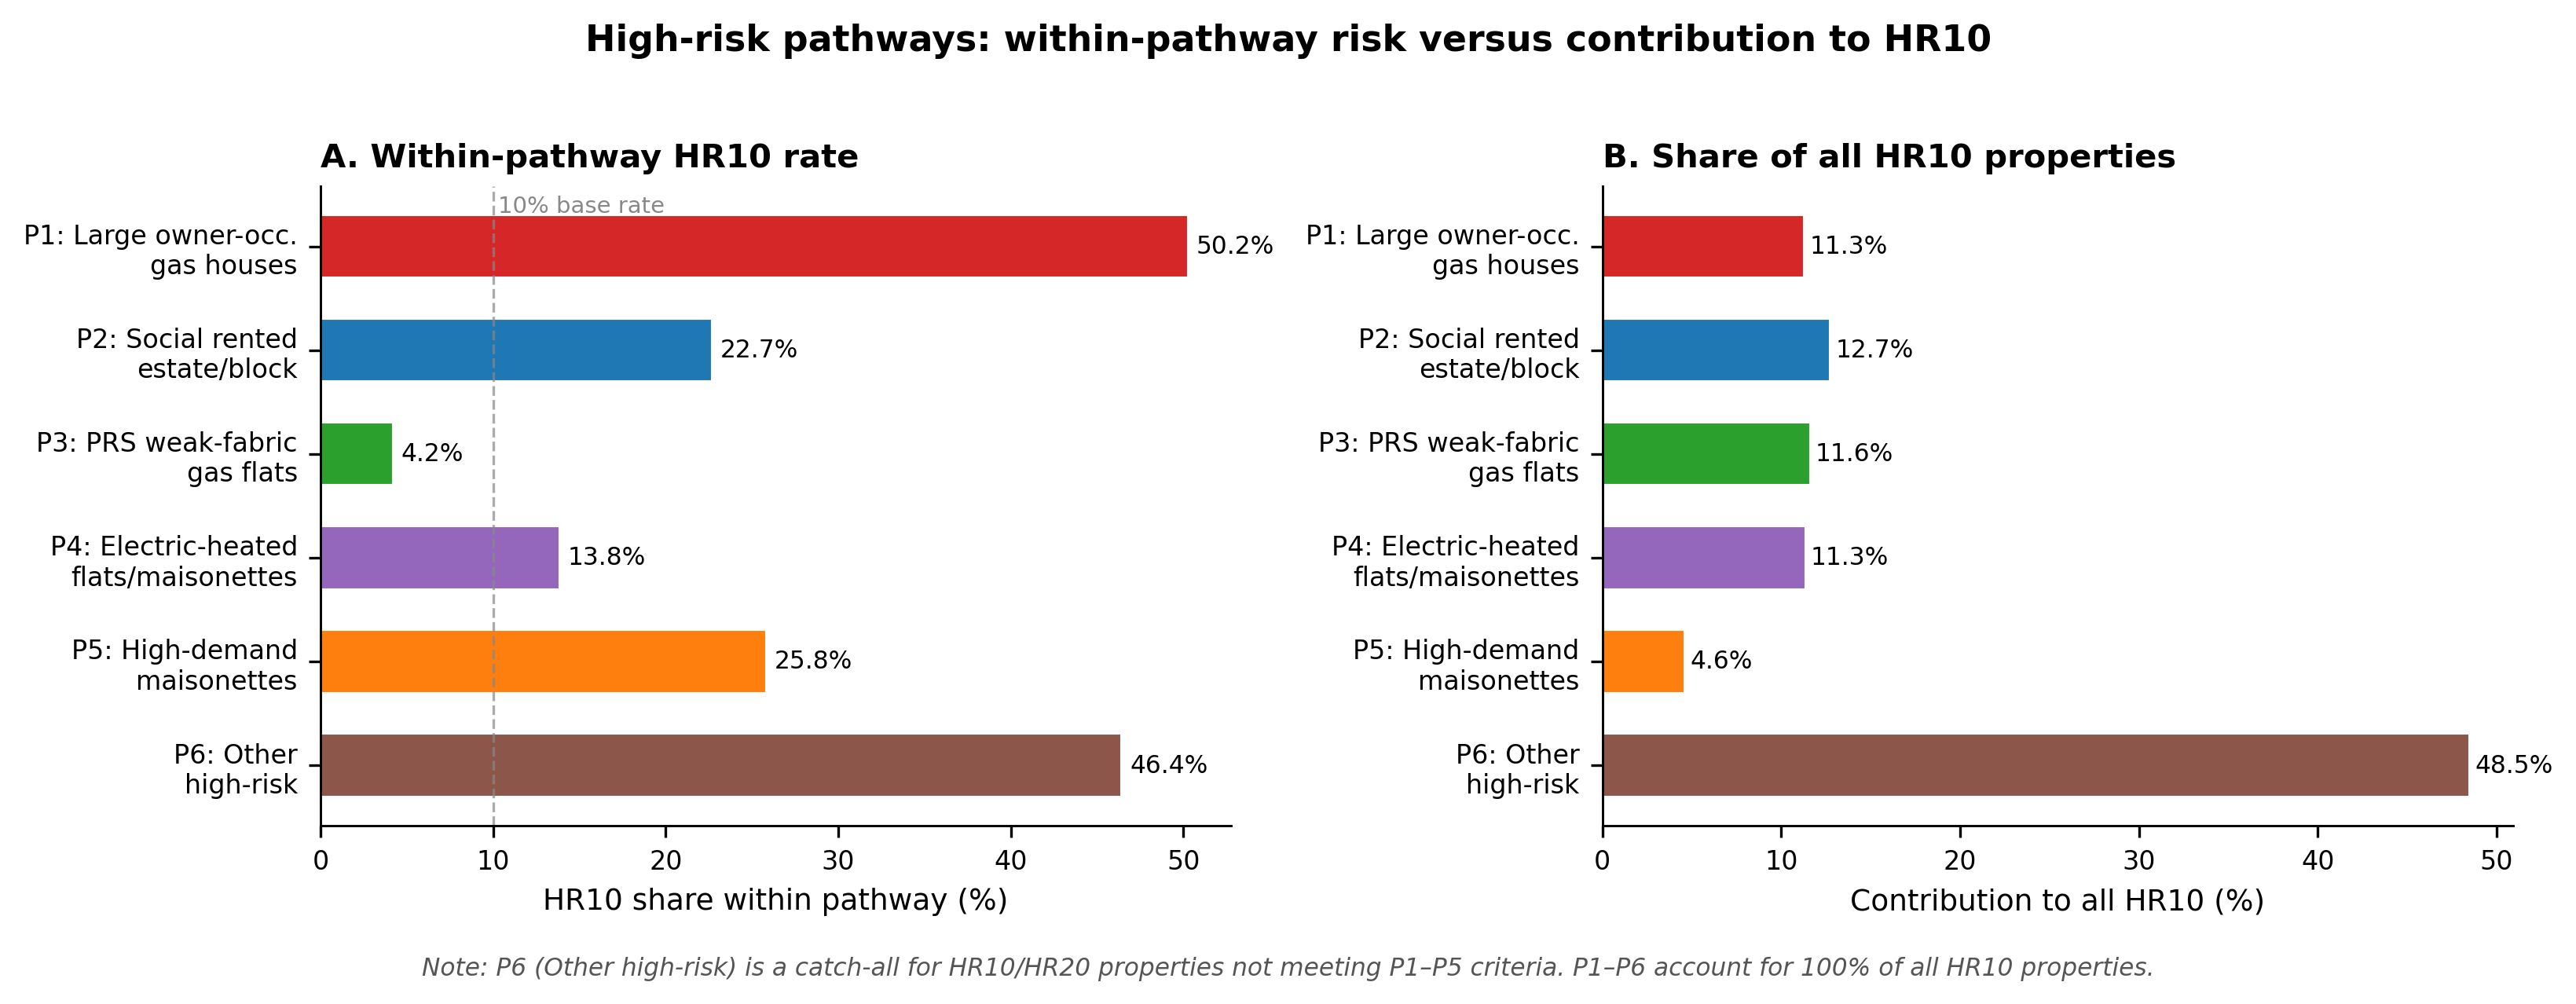
\includegraphics[width=\linewidth]{paper/figures/high_risk_pathway_contribution.png}
\caption{Within-pathway HR10 risk and contribution to all HR10 properties. The figure distinguishes intensity from scale: some pathways have high within-group exposure, while others contribute substantially because they are more numerous in the Westminster stock.}
\label{fig:high-risk-pathway-contribution}
\end{figure}

\begin{figure}[H]
\centering
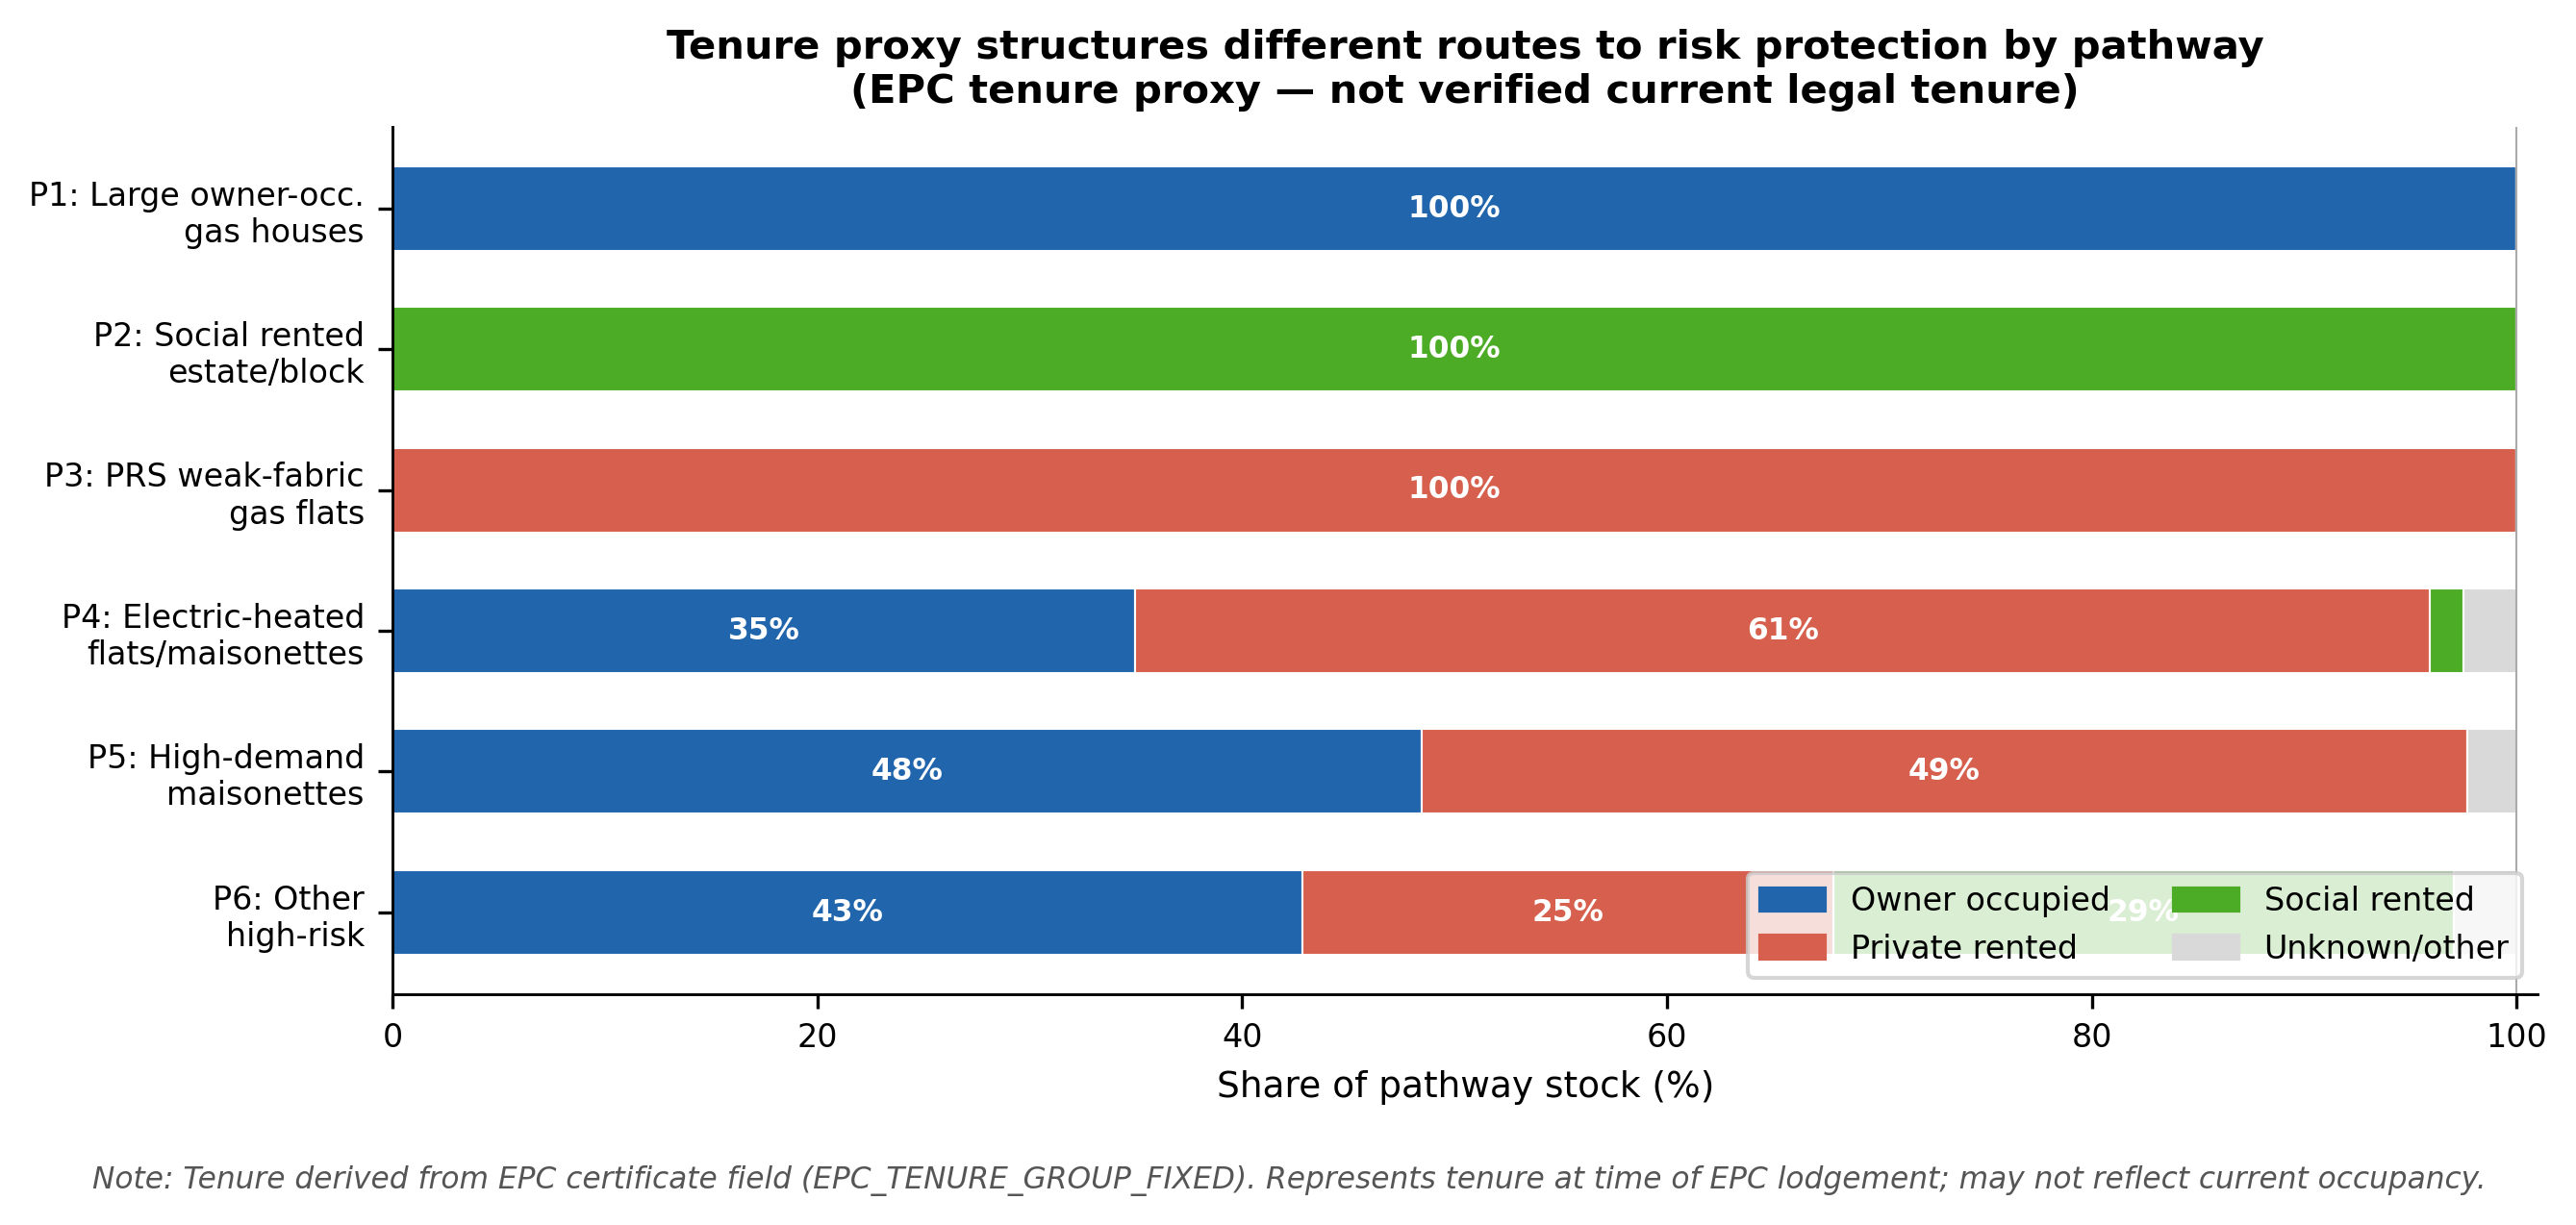
\includegraphics[width=0.92\linewidth]{paper/figures/high_risk_tenure_by_pathway.png}
\caption{Tenure-proxy composition by high-risk pathway. The figure links each descriptive pathway to a different governance route, including owner-occupation, social housing delivery, private rented enforcement, and mixed residual cases.}
\label{fig:tenure-by-pathway}
\end{figure}

Figure~\ref{fig:tenure-by-pathway} then shows why these pathways imply different governance routes, rather than a single retrofit-delivery model. The electric-exposure comparison in Figure~\ref{fig:electric-exposure} isolates inefficient flats and maisonettes with EPC-recorded electricity exposure from non-electric low-EPC comparators and the remaining stock. Its purpose is not to claim that electrification causes high burden, but to show why household-facing electricity prices, fabric quality, and tariff access must be modelled before clean heat can be interpreted as price-risk protection.

\begin{figure}[H]
\centering
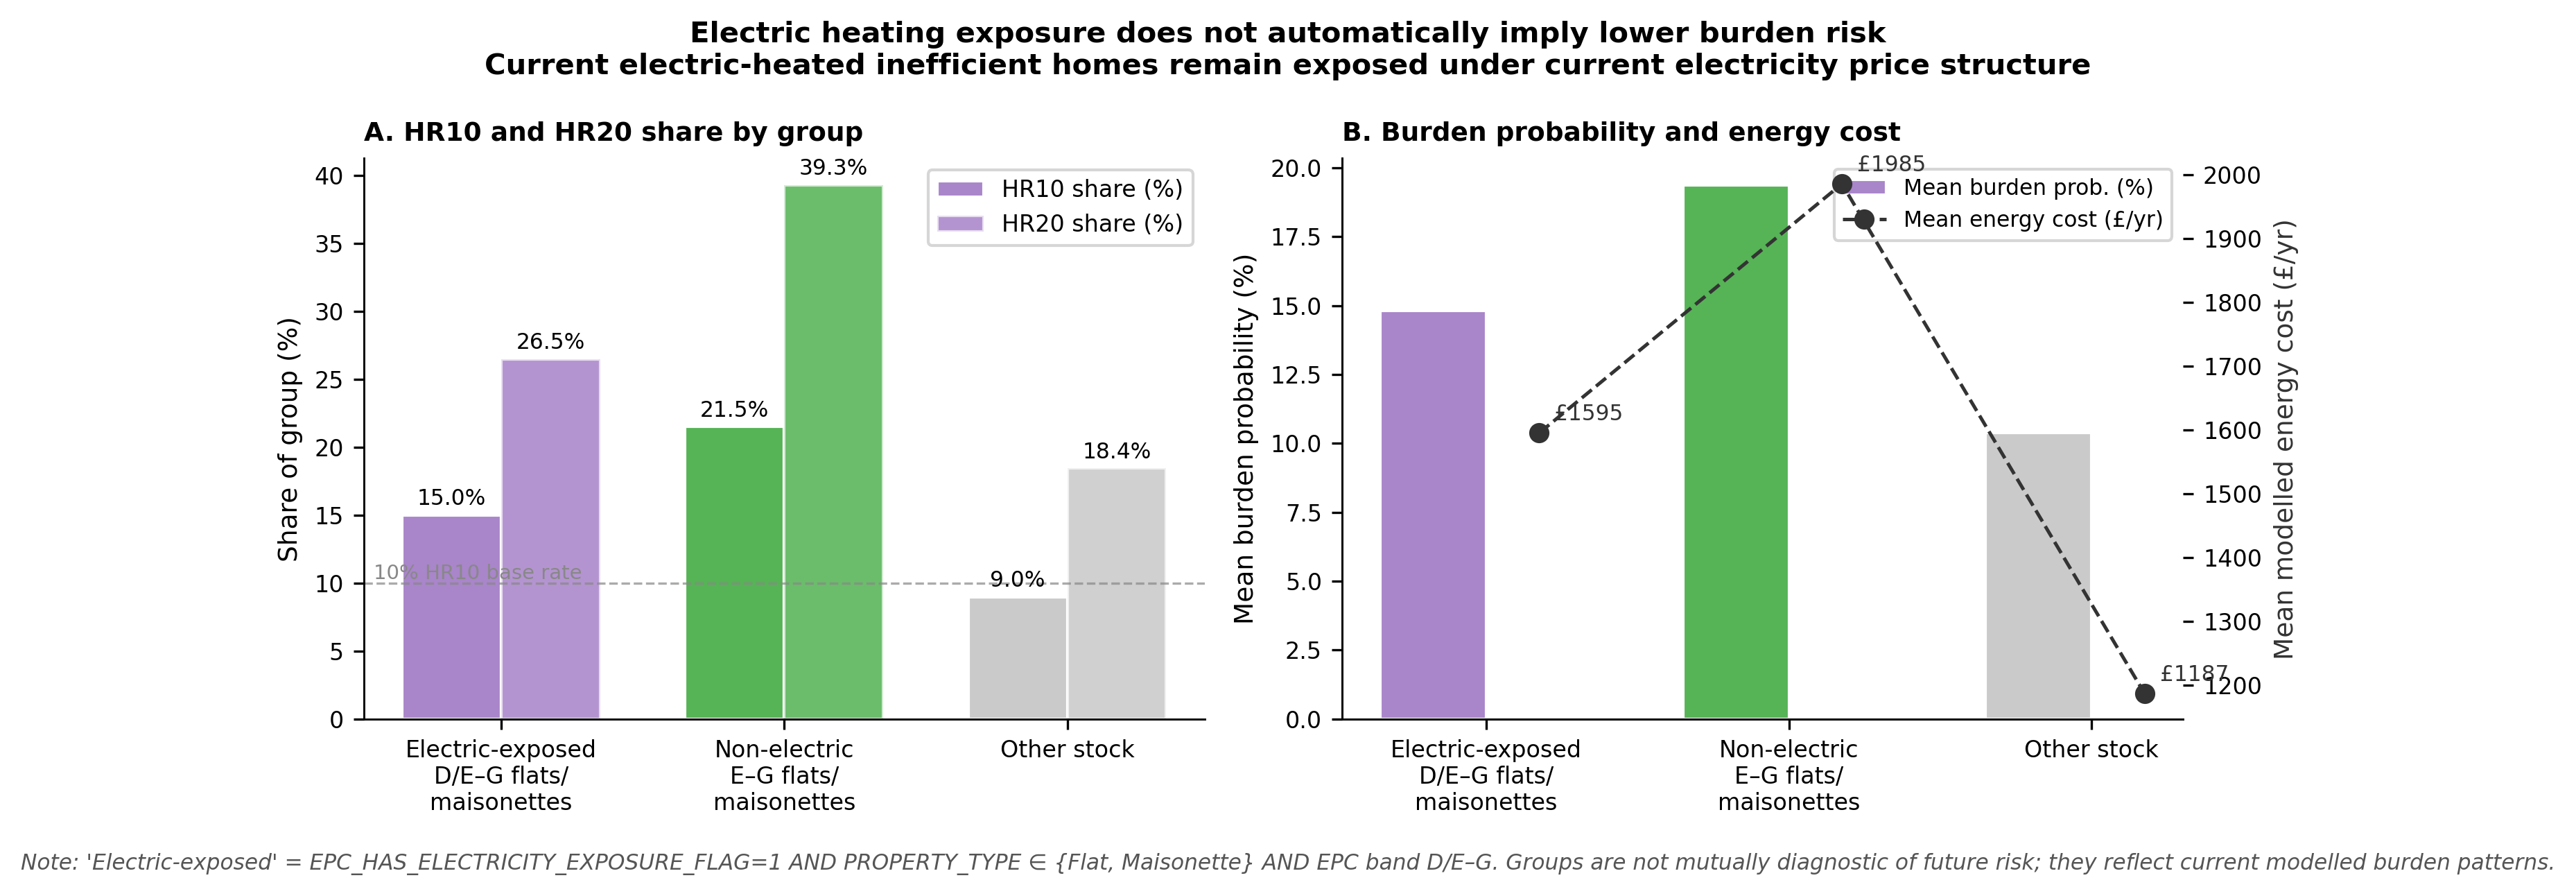
\includegraphics[width=\linewidth]{paper/figures/high_risk_electric_exposure.png}
\caption{Current burden exposure among electric-exposed inefficient flats and maisonettes compared with non-electric low-EPC flats and the rest of the stock. The figure supports the paper's caution that electricity exposure and electrification are not automatically household de-risking mechanisms under current price structures.}
\label{fig:electric-exposure}
\end{figure}

The spatial outputs in Figure~\ref{fig:spatial-high-risk} show that Westminster's current high-burden exposure is geographically uneven and mechanism-specific. They should be interpreted as LSOA-level descriptive maps of current HR10 concentration and dominant HR10 pathway, not as direct maps of future price-shock risk.

\begin{figure}[H]
\centering
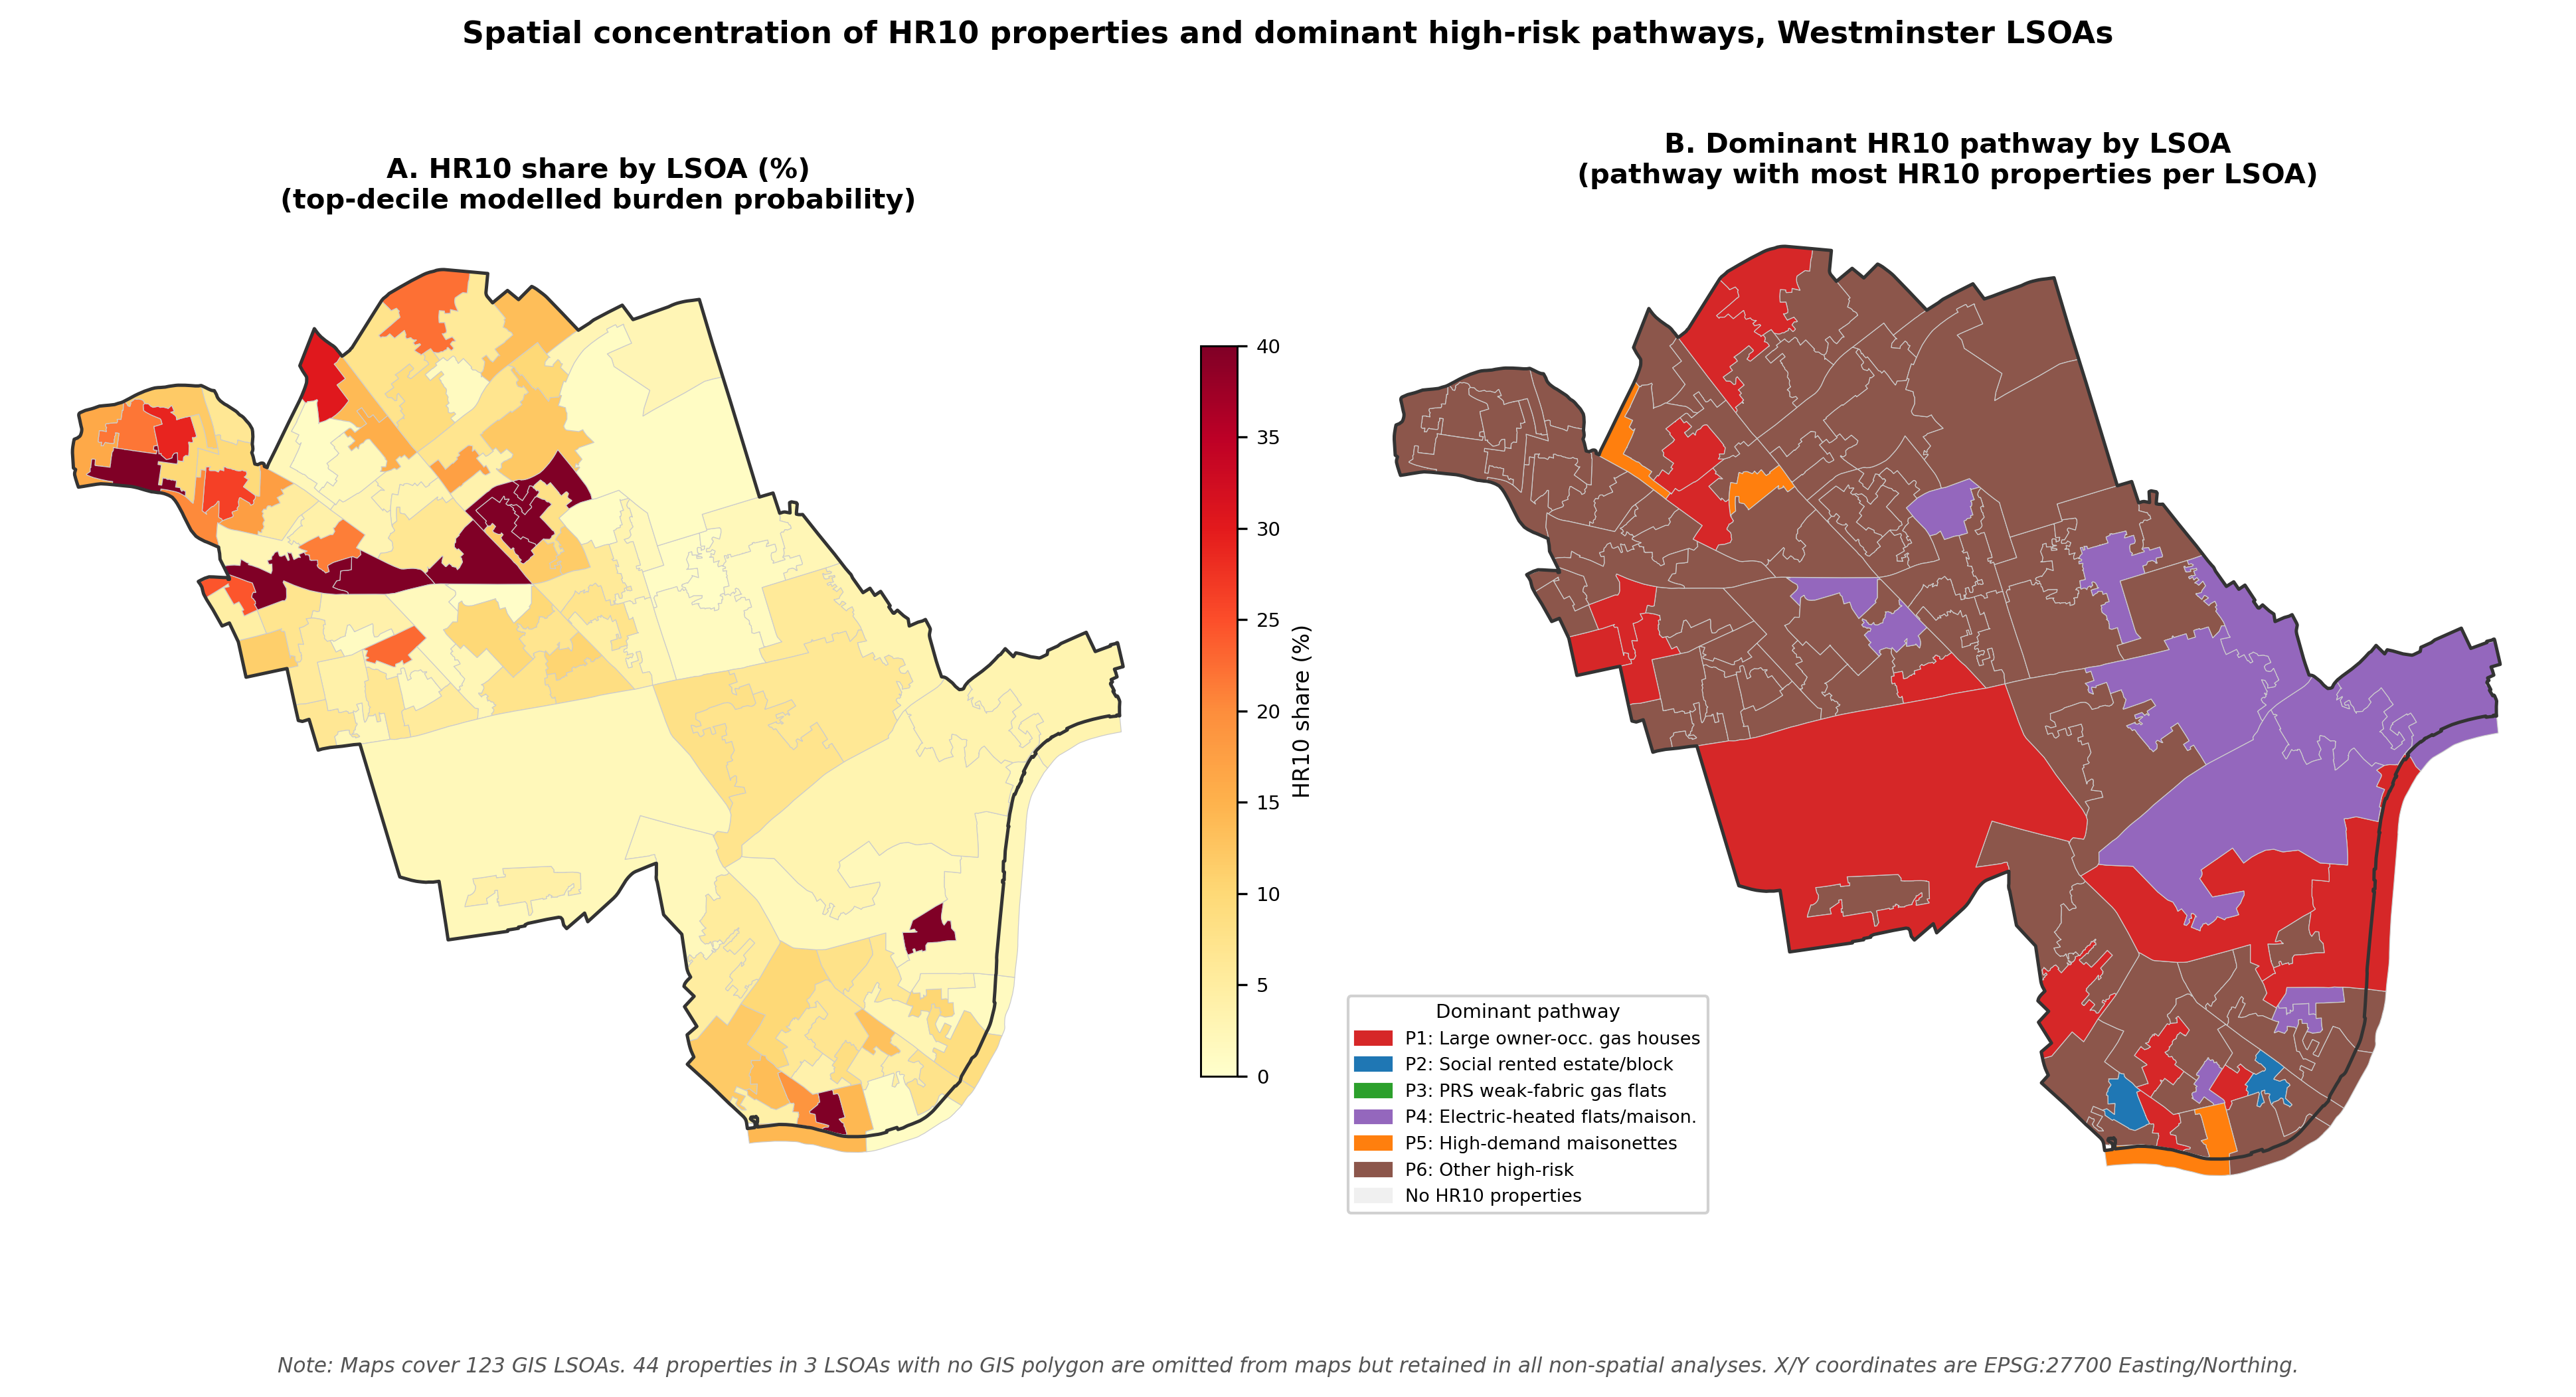
\includegraphics[width=\linewidth]{paper/figures/high_risk_spatial_maps.png}
\caption{Spatial concentration of current modelled HR10 exposure in Westminster. Panel A maps the LSOA share of properties in HR10; Panel B maps the dominant high-risk pathway among HR10 properties in each LSOA. The maps use the 123 LSOAs available in the GIS boundary file.}
\label{fig:spatial-high-risk}
\end{figure}

The residual group is especially important for the next stage. It is too large to remain a black-box category once the paper moves from current exposure into price-shock risk. The planned analysis should separate income-driven residual cases, spatial-deprivation concentrations, mixed housing-and-income mechanisms, and unusual dwelling profiles. This will help distinguish households for whom technical retrofit is the central risk-reduction route from those for whom social tariffs, standing-charge reform, income support, or local assistance may be more relevant.

\subsection{Implemented Official Price-Spine Outputs}

The official price-spine construction adds the price input layer for the next empirical stage. The imported materials report a London monthly domestic spine with 94 S0--S6 rows, an event-level London spine with 22 rows, an all-region Ofgem parser audit, a road-fuel appendix, and a QA summary with no failed checks. These outputs are analytically useful because they allow the paper to model price shocks as specific retail pass-through structures rather than as generic percentage increases. They do not yet estimate household fuel price risk, because required demand, residual income, payment method, fuel connection, and intervention feasibility still need to be joined to the price layer.

Figures~\ref{fig:official-price-spine-timeline}--\ref{fig:official-price-spine-s6} are therefore promoted as method figures. Figure~\ref{fig:official-price-spine-timeline} documents the temporal architecture of S0--S6; Figure~\ref{fig:official-price-spine-unit-rates} shows the unit-rate progression and the S3/S4 policy-buffering contrast; Figure~\ref{fig:official-price-spine-decomposition} keeps unit-rate and standing-charge exposure visible; and Figure~\ref{fig:official-price-spine-s6} identifies the fixed-cost sensitivity that should be interpreted with the documented Q3 proxy caveat. Together, these figures support the scenario engine that will generate burden uplift, threshold crossing, Fuel Price-at-Risk, and de-risking dividends in the next modelling layer.

\subsection{Implemented Price-Shock Result Outputs}

The first price-shock result layer now converts the baseline engine and official price spine into paper-facing evidence on burden uplift and threshold-crossing risk. These outputs use Direct Debit as the central payment-method track and treat Standard Credit and Prepayment as sensitivity tracks until observed household payment-method data are available. The main results focus on S3, S4, and S6 Q3, with S0 and S2 retained as scenario-profile anchors. They should be read as price-shock results, not yet as intervention results: formal Household Fuel Price-at-Risk, affordability gap-at-risk, and de-risking dividend calculations remain the next modelling layer.

Figure~\ref{fig:shock-mechanism-heatmaps} establishes the structural mechanism of exposure under the S3 unmitigated shock. Gas-heated E--G dwellings have a weighted mean required-energy burden uplift of about 10.0 percentage points, compared with about 2.8 percentage points for electricity-heated A--C dwellings. The dwelling-form panel shows a further amplification: E--G houses reach about 12.6 percentage points, while E--G flats are closer to 7.0 percentage points. The result is not simply that inefficient homes are expensive; it is that fuel, fabric, and dwelling form jointly shape price sensitivity.

\begin{figure}[H]
\centering
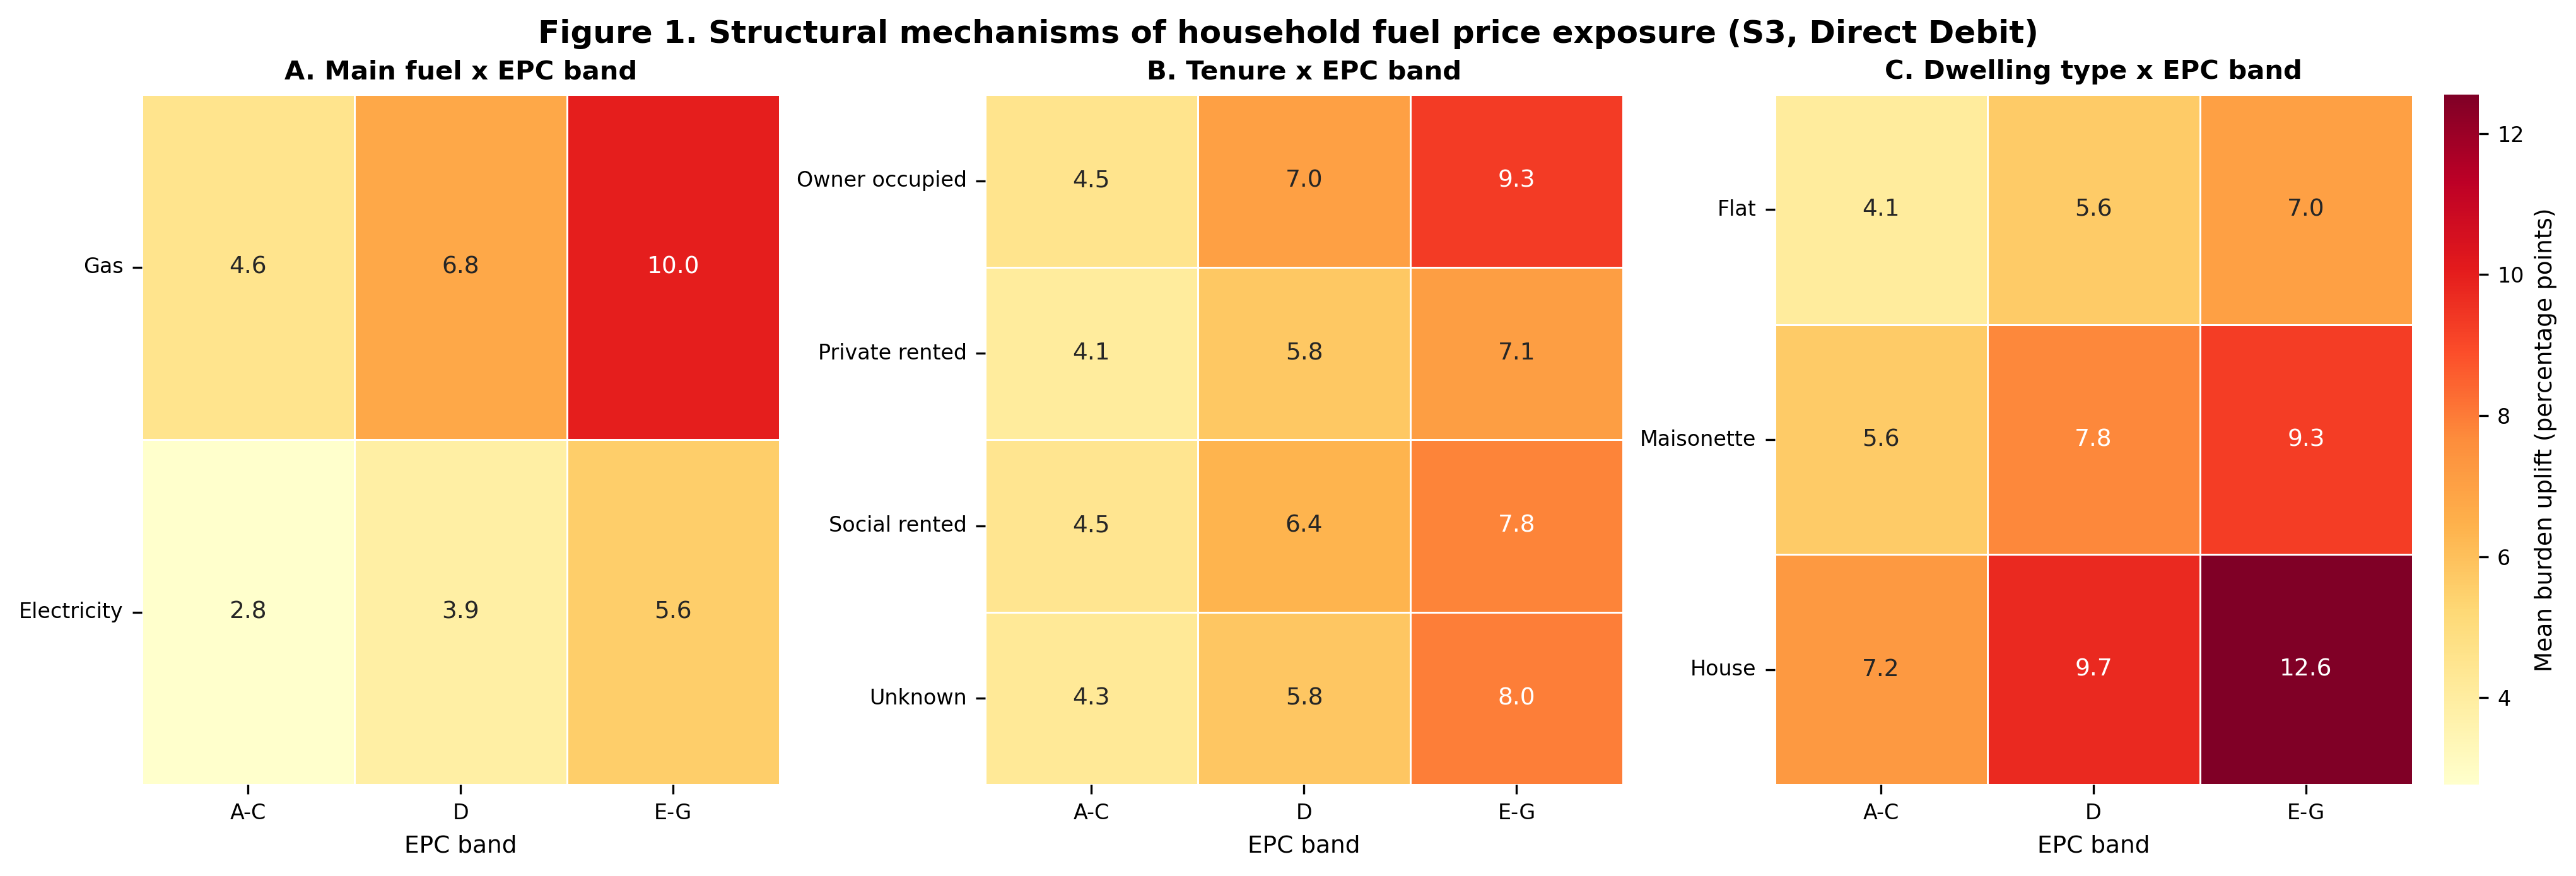
\includegraphics[width=\linewidth]{paper/figures/fuel_price_shock_mechanism_heatmaps.png}
\caption{Weighted mean required-energy burden uplift under the S3 unmitigated price shock, by Westminster dwelling and household-dwelling characteristics. Values are percentage-point changes relative to S0, using Direct Debit as the central payment-method track.}
\label{fig:shock-mechanism-heatmaps}
\end{figure}

Figure~\ref{fig:shock-top-archetypes} then identifies the most exposed household-dwelling archetypes. The highest S3 burden-uplift groups are dominated by gas-heated houses and maisonettes with weak EPC performance. Owner-occupied houses in EPC E--G with gas heating have an average burden uplift of about 13.9 percentage points and a threshold-crossing probability of about 86.7\%; private rented houses in EPC E--G with gas heating follow at about 11.8 percentage points and 81.4\%. The ranking therefore moves the paper beyond generic statements about vulnerable households: exposure is concentrated in specific tenure--dwelling--fabric--fuel combinations.

\begin{figure}[H]
\centering
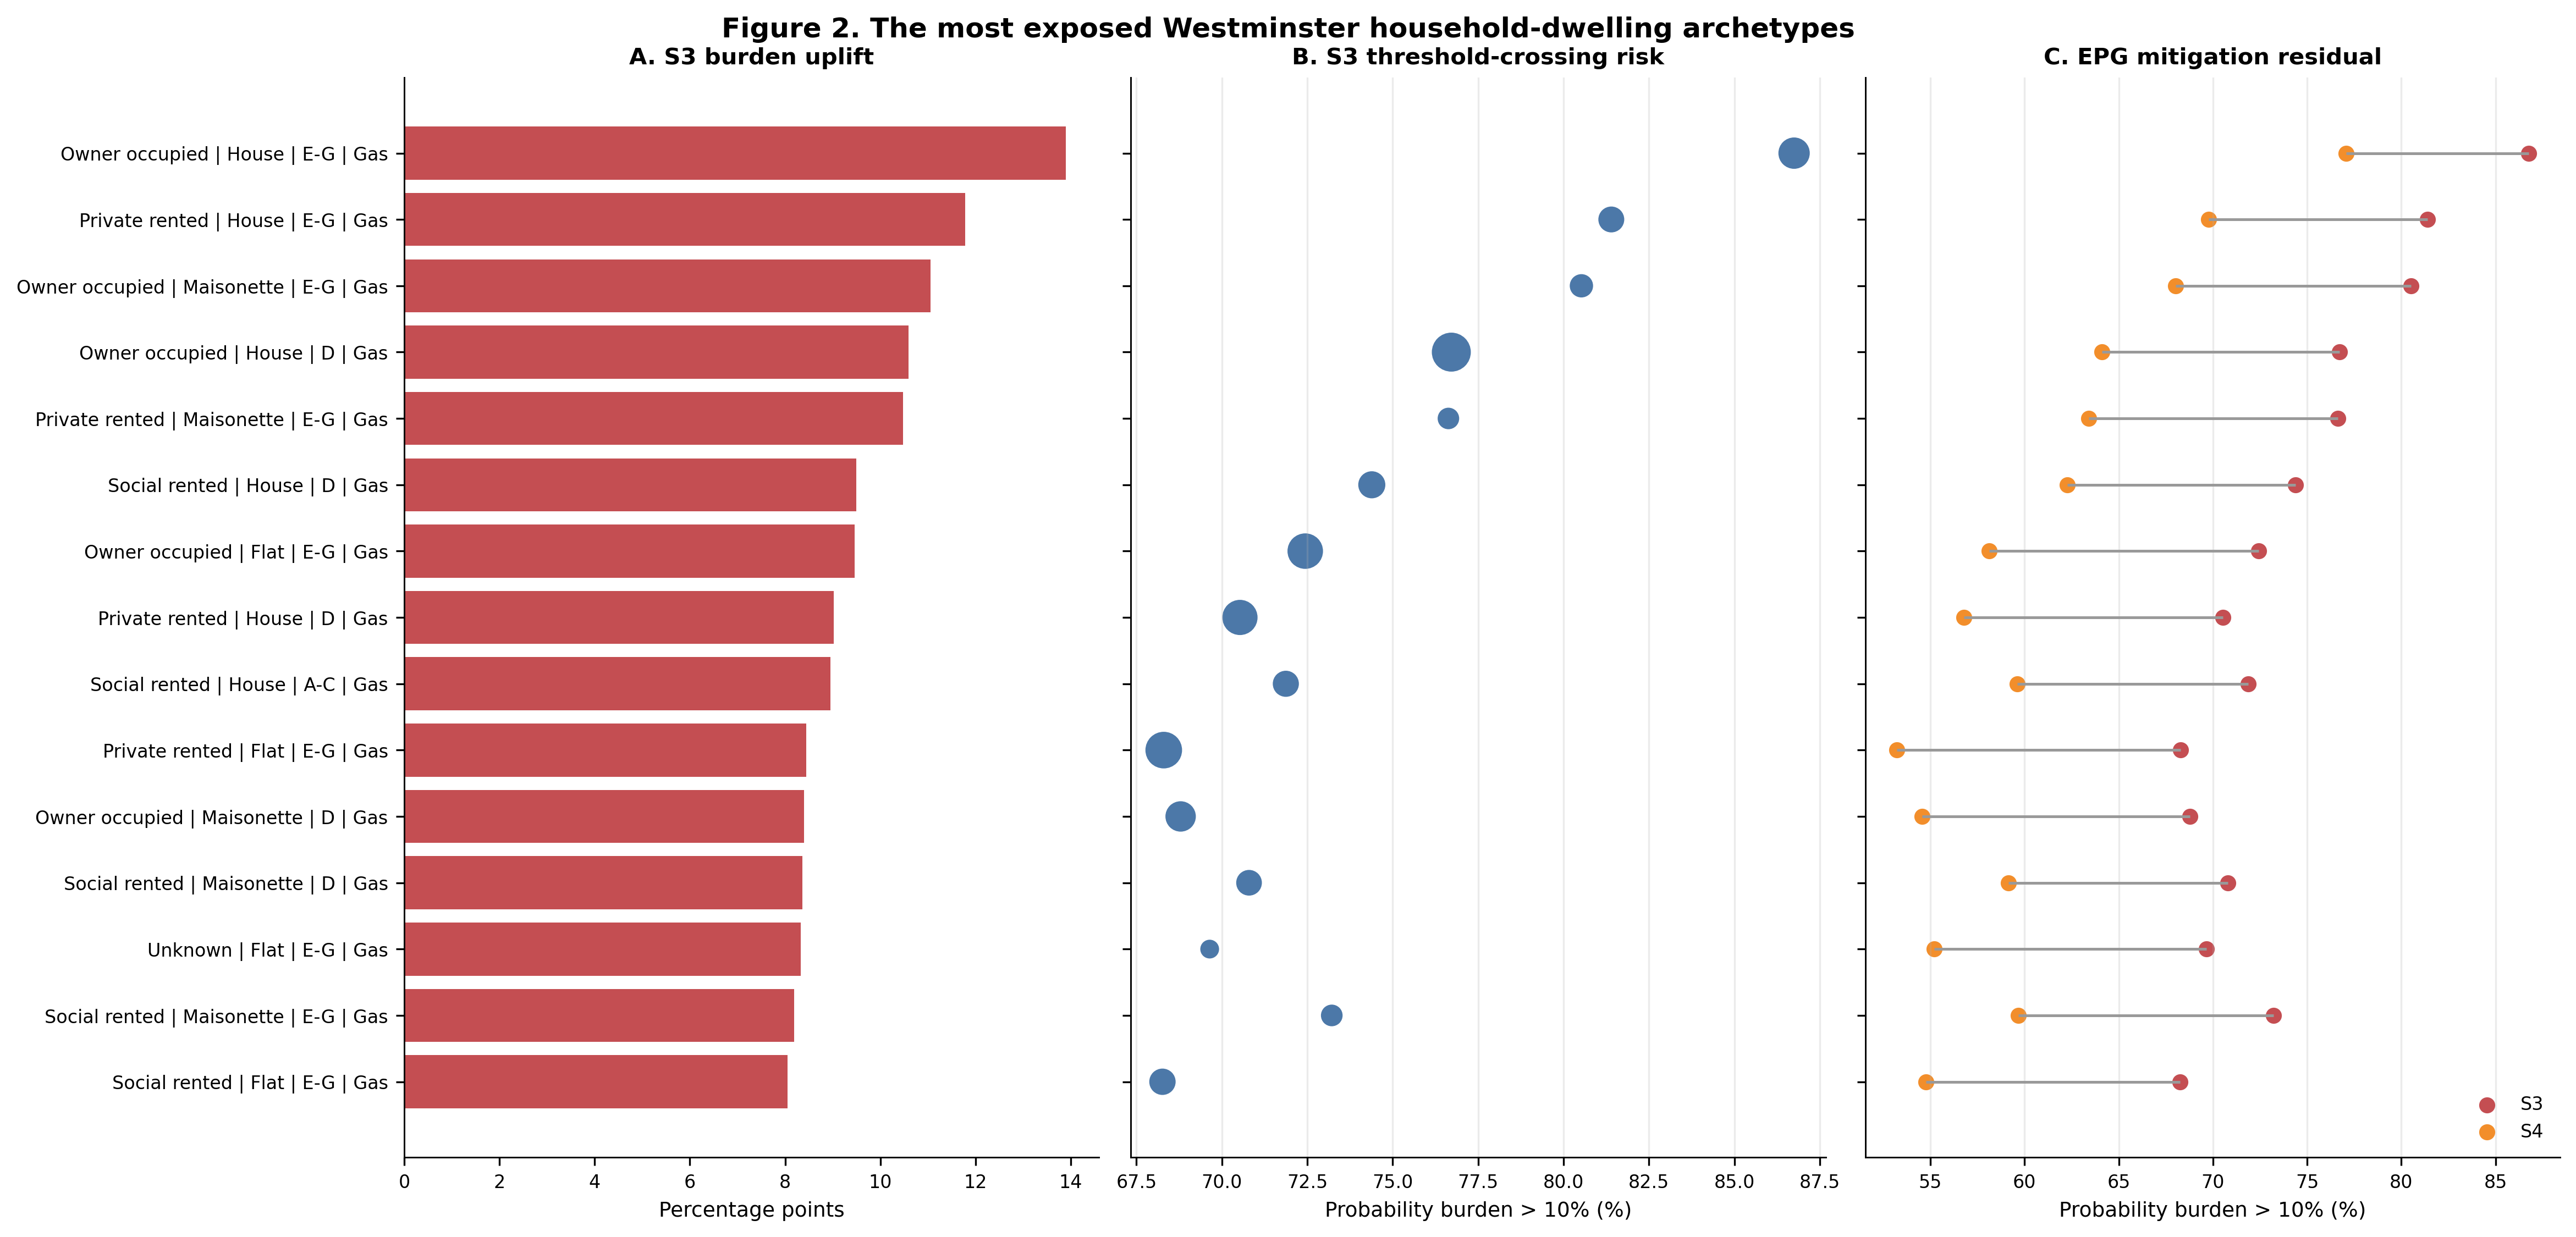
\includegraphics[width=\linewidth]{paper/figures/fuel_price_shock_top_archetype_ranking.png}
\caption{Top Westminster household-dwelling archetypes ranked by S3 required-energy burden uplift, with corresponding S3 threshold-crossing risk and policy-mitigated residual exposure under S4. Archetypes are included where the weighted summary contains at least 100 records.}
\label{fig:shock-top-archetypes}
\end{figure}

Figure~\ref{fig:shock-scenario-profiles} shows how scenario design changes group-level risk. S3 creates a clear risk peak across EPC, fuel, and tenure groups; S4 reduces this exposure through the Energy Price Guarantee; and S6 Q3 leaves a residual fixed-cost and tariff-structure sensitivity. For EPC E--G dwellings, the threshold-crossing probability is about 66.0\% under S3, 51.4\% under S4, and 40.2\% under S6 Q3. The profile supports the paper's distinction between market exposure and policy buffering: mitigation lowers risk but does not remove the underlying inequality in exposure.

\begin{figure}[H]
\centering
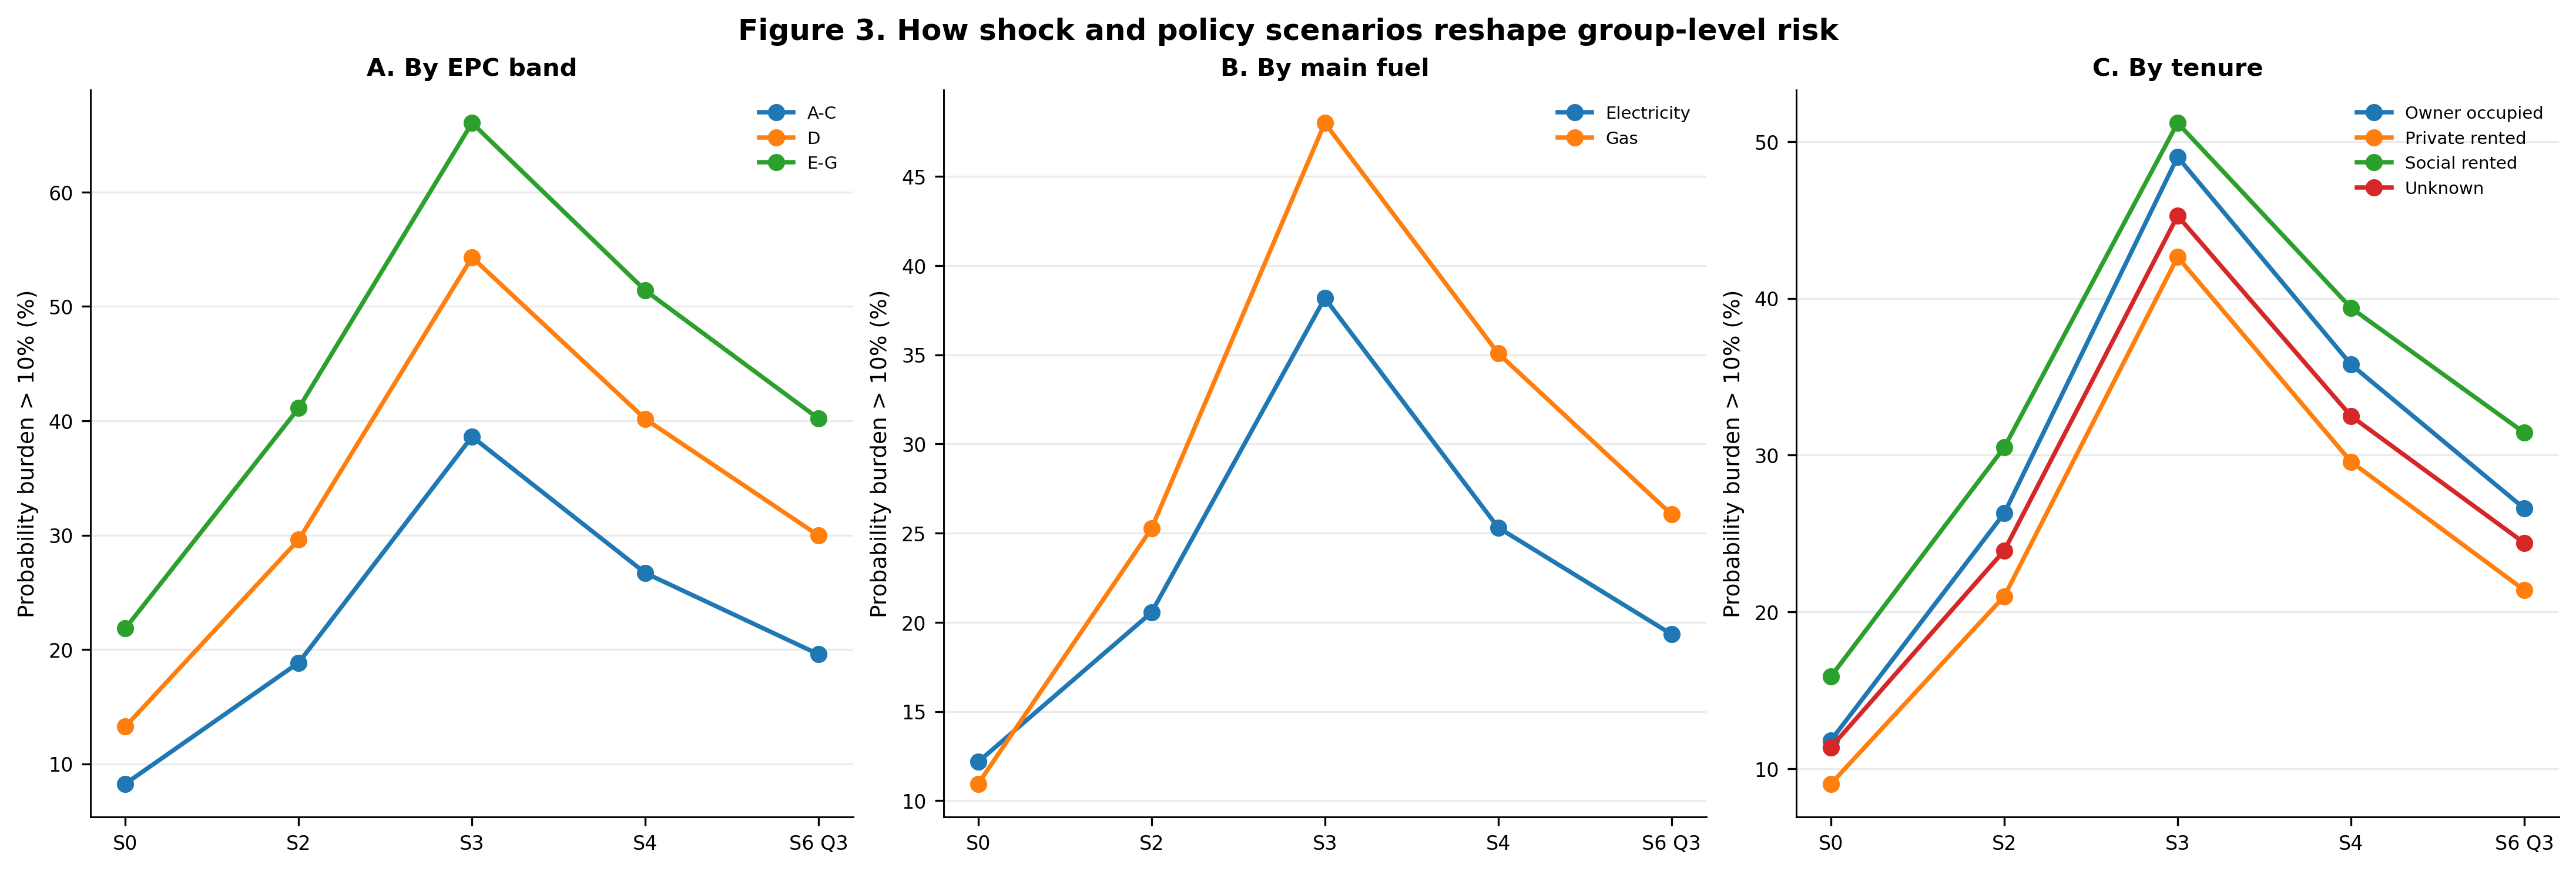
\includegraphics[width=\linewidth]{paper/figures/fuel_price_shock_scenario_response_profiles.png}
\caption{Threshold-crossing probability across S0, S2, S3, S4, and S6 Q3, showing how unmitigated shocks, policy mitigation, and tariff-structure sensitivity reshape group-level household fuel price risk.}
\label{fig:shock-scenario-profiles}
\end{figure}

Finally, Figure~\ref{fig:shock-spatial-distribution} shows that the price-shock burden is spatially concentrated within Westminster. The highest S3 threshold-crossing probabilities in the mapped LSOAs are around 70--76\%, while the diagnostic scatter shows that baseline threshold risk and S3 burden uplift are related but not identical. This spatial result should be interpreted as required-energy price-risk concentration, not as a direct map of observed current fuel poverty. The map uses the 123 LSOAs available in the current GIS boundary file; the three unmatched result LSOAs are retained in non-spatial summaries but omitted from the mapped panels.

\begin{figure}[H]
\centering
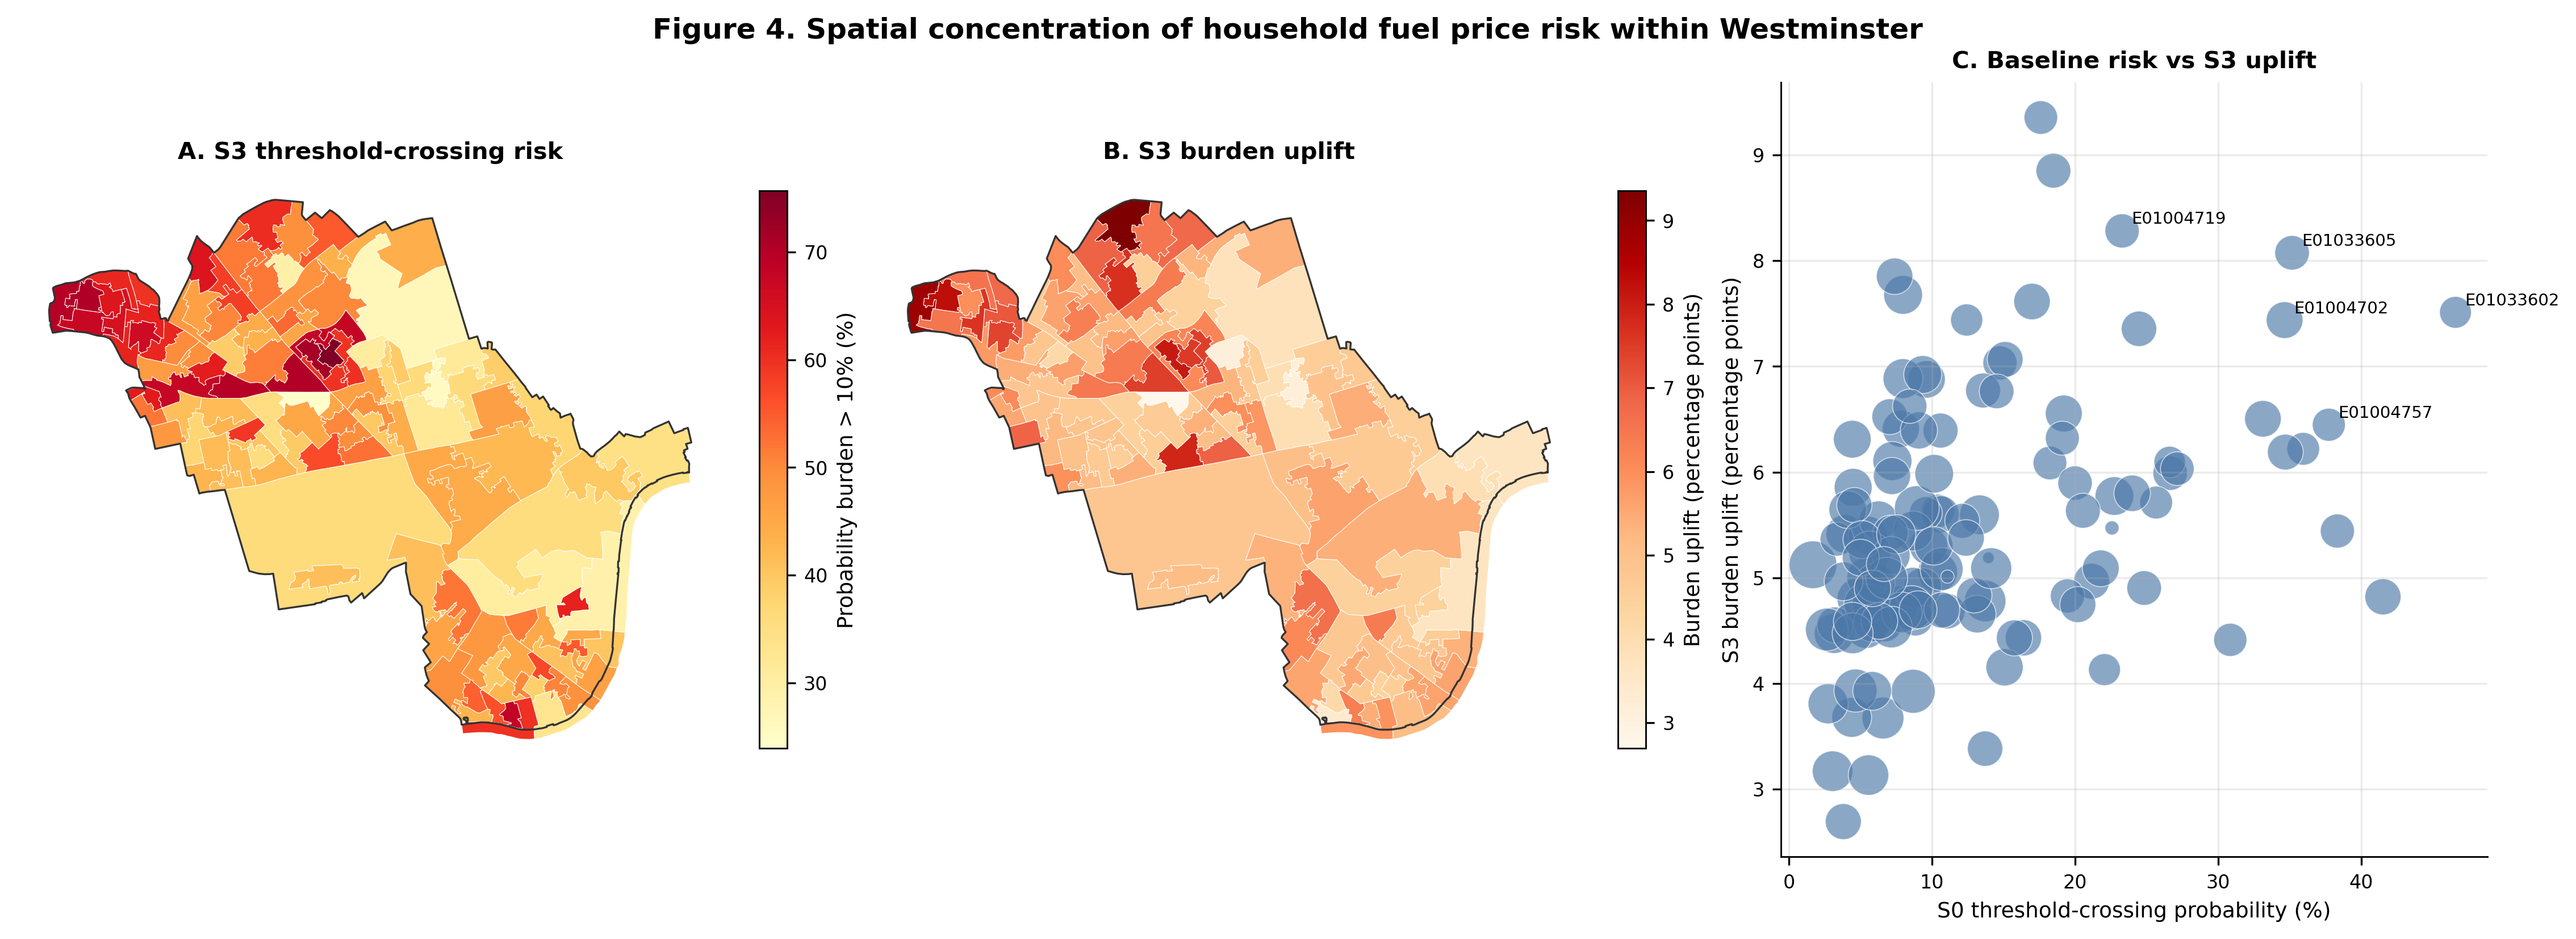
\includegraphics[width=\linewidth]{paper/figures/fuel_price_shock_spatial_distribution.png}
\caption{Spatial concentration of S3 household fuel price risk across Westminster LSOAs. The maps show threshold-crossing probability and required-energy burden uplift; the scatter compares baseline threshold risk with S3 burden uplift.}
\label{fig:shock-spatial-distribution}
\end{figure}

\subsection{Planned Intervention Outputs}

The next empirical layer will estimate intervention-specific protection against the implemented price-shock results. It will compare fabric retrofit, clean heat, PV, battery storage, smart tariffs, and integrated packages under explicit assumptions about technical feasibility, tenure and leasehold governance, roof access, tariff access, electricity/gas price ratios, and policy support. The paper will report not only average burden changes, but also upper-tail risk, burden uplift, threshold-crossing probabilities, and the probability that households remain above policy-relevant burden thresholds after intervention.

The scenario engine should continue to use the baseline extract's applicability fields rather than joining every property to every price scenario. Gas and electricity properties enter S0--S4 and S6 with Direct Debit, Standard Credit, and Prepayment sensitivity labels; oil properties enter only the S5 heating-oil sensitivity. Payment method should remain a scenario dimension unless observed household payment data are added later. This prevents the results from overstating precision or misclassifying oil-heated properties as if they were regulated mains-gas or mains-electricity tariff-cap cases.

A central planned output is the de-risking dividend:
\begin{equation}
\text{De-risking dividend} = \text{Fuel Price-at-Risk}_{\text{before}} - \text{Fuel Price-at-Risk}_{\text{after}}.
\end{equation}
This metric will be estimated by intervention package and household-dwelling condition, including fabric retrofit, clean heat, PV, battery storage, smart tariffs, and integrated packages. Its interpretation will remain conditional: an intervention produces household price-risk protection only where technical feasibility, tenure and leasehold governance, tariff access, electricity/gas price ratios, and market pass-through allow the engineering change to reduce household exposure.

\subsection{Figures and Tables}

Expected tables will summarise baseline burden probabilities, modelled fuel-poverty diagnostics, price-shock burden uplift, Fuel Price-at-Risk, and intervention-specific de-risking dividends by income group, EPC rating, dwelling form, heating system, tenure, payment method, and LSOA/MSOA. The baseline extract figures now promoted into the manuscript are Figures~\ref{fig:baseline-burden-distribution}--\ref{fig:baseline-high-burden-main-fuel}; the current high-risk explanation figures are Figures~\ref{fig:hr-br-overlap}--\ref{fig:spatial-high-risk}; the official price-spine figures are Figures~\ref{fig:official-price-spine-timeline}--\ref{fig:official-price-spine-s6}; and the first price-shock result figures are Figures~\ref{fig:shock-mechanism-heatmaps}--\ref{fig:shock-spatial-distribution}. Remaining expected figures will include: the conceptual distinction between fuel poverty, energy burden, and household fuel price risk; intervention de-risking comparisons; and maps of de-risking gaps.

Before intervention results are reported, the spatial outputs should establish whether different mechanisms concentrate in different parts of Westminster. Priority maps include LSOA HR10 share, LSOA HR20 share, dominant HR10 pathway, social rented estate/block concentration, electric-heated inefficient flat concentration, and residual high-risk concentration. These maps would support the paper's claim that fuel price risk is produced by locally specific combinations of housing form, income sensitivity, and governance constraints rather than by a uniform borough-wide condition.

The synced LSOA income PDF panels from the latest run are included above as Figures~\ref{fig:lsoa-income-pdf-scenarios-1}--\ref{fig:lsoa-income-pdf-scenarios-3}. They show the estimated lognormal income distributions under selected $\lambda$ values, with poverty-line and MSOA-mean markers. They are captioned as synthetic constrained income distributions for burden modelling, not as observed household income distributions and not as direct household fuel price risk outputs.

The paper will ultimately identify de-risking gaps: places and household-dwelling types where fuel price protection is most needed but low-carbon intervention is least accessible. These gaps are expected to be especially important where Westminster's high housing costs, private renting, leasehold flats, heritage constraints, district-heating governance, and uneven tariff or asset access interrupt the translation from domestic net zero investment into household price-risk protection.

\section{Discussion}

The expected policy implication is that domestic net zero should be treated as a distributional household risk-protection agenda. Protection depends on the alignment of fabric retrofit, heating technology, distributed generation, flexibility, tariff design, electricity market reform, capital access, and tenure-sensitive governance.

In Westminster, this means paying particular attention to private renters, leasehold flats, HMOs, heritage-constrained dwellings, district-heating governance, social housing delivery pathways, and households whose vulnerability is masked by high neighbourhood average wealth.

\section{Conclusion}

Fuel poverty identifies current hardship; household fuel price risk identifies future exposure to price shocks. Net zero determines who receives protection only when domestic interventions are technically effective, financially accessible, and institutionally deliverable for the households most exposed.

The paper therefore asks not whether net zero reduces emissions, but whether, how, and for whom it credibly reduces household exposure to fossil-fuel price volatility.


% Enable when references.bib contains cited entries.
% \bibliographystyle{apalike}
% \bibliography{references}

\end{document}
